\NoBgThispage
\chapter{MapAlign: deep-Learning based approach}

\section{Neural Networks}
Neural networks (NNs) are computational models inspired by the structure and functionality of the human brain, consisting of interconnected layers of neurons. Just as biological neurons process signals transmitted across synapses, artificial neurons in a neural network receive inputs, process them, and generate outputs \cite{Grosan2011}. These networks are primarily used in a wide range of machine learning tasks such as image recognition, natural language processing, and predictive analytics.
In this chapter the building blocks, main principles, and training methodologies of neural networks will be explored, starting with an in-depth discussion of the neuron as the basic unit.

\subsection{Neuron and its Function}
At the core of every neural network lies the artificial neuron, modeled after its biological counterpart. Each neuron receives input signals, which are processed and combined to produce an output. Mathematically, this process is represented as follows \cite{10.11648/j.ajnna.20190501.12}:
% Neuron Input
\begin{equation}
    \textit{net}_i = \sum_{j=1}^{d} w_{ji} \cdot \textit{in}_j + w_{0i}
\end{equation}


Here, $(\text{in}_1, \text{in}_2, \ldots, \text{in}_d)$ are the $d$ inputs the neuron receives, analogous to signals received by biological neurons through synapses. These inputs are weighted by $w_{ji}$, which are the synaptic weights, representing the strength of the connection between neurons, which can be either positive (if one
unit excites another) or negative (if one unit suppresses or
inhibits another). The higher the weight, the more influence
one unit has on another. (This corresponds to the way actual
brain cells trigger one another across tiny gaps called synapses) \cite{10.11648/j.ajnna.20190501.12}.

Learning in a neural network is essentially an adjustment of these weights. The term $w_{0i}$ is a bias that helps adjust the output and enhances the model's flexibility. The sum of these weighted inputs results in the neuron’s excitation level, denoted as $\textit{net}_i$.
Once the net input ${net}_i$ is computed, the neuron applies an activation function $f(\cdot)$ to determine the output:
% Neuron Output
\begin{equation}
    \textit{out}_i = f(\textit{net}_i)
\end{equation}

\begin{figure}
    \centering
    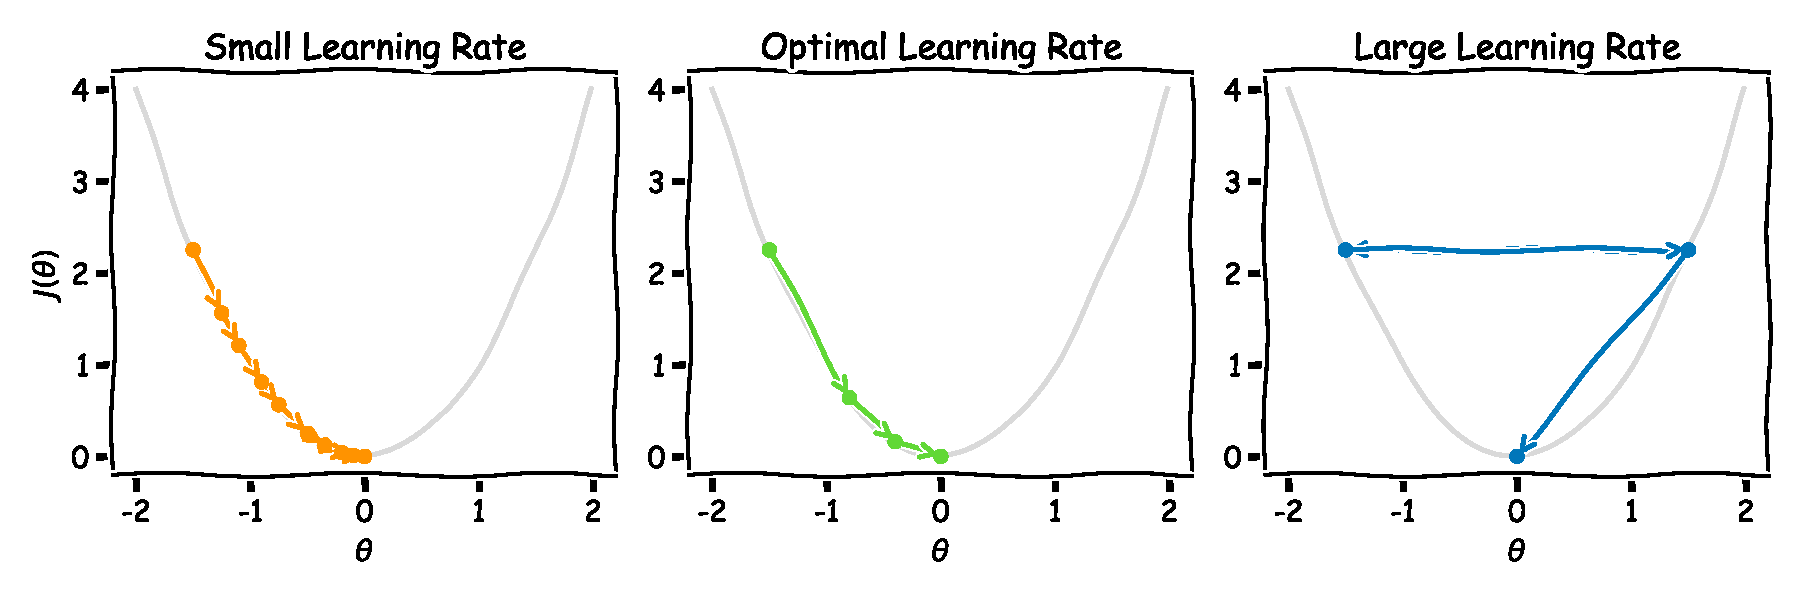
\includegraphics[width=1\linewidth]{LateX//figs/learning_rate.pdf}
    \caption{Enter Caption}
    \label{fig:enter-label}
\end{figure}


The activation function introduces non-linearity to the model, enabling neural networks to learn complex, non-linear mappings between inputs and outputs. Common activation functions include:
\begin{itemize}
    \item Sigmoid: Outputs values between $0$ and $1$.
    \item Tanh: Outputs values between $-1$ and $1$.
    \item ReLU: Outputs values following: $f(\textit{net}_i) = \max(0, \textit{net}_i)$.
\end{itemize}

\begin{figure}
    \centering
    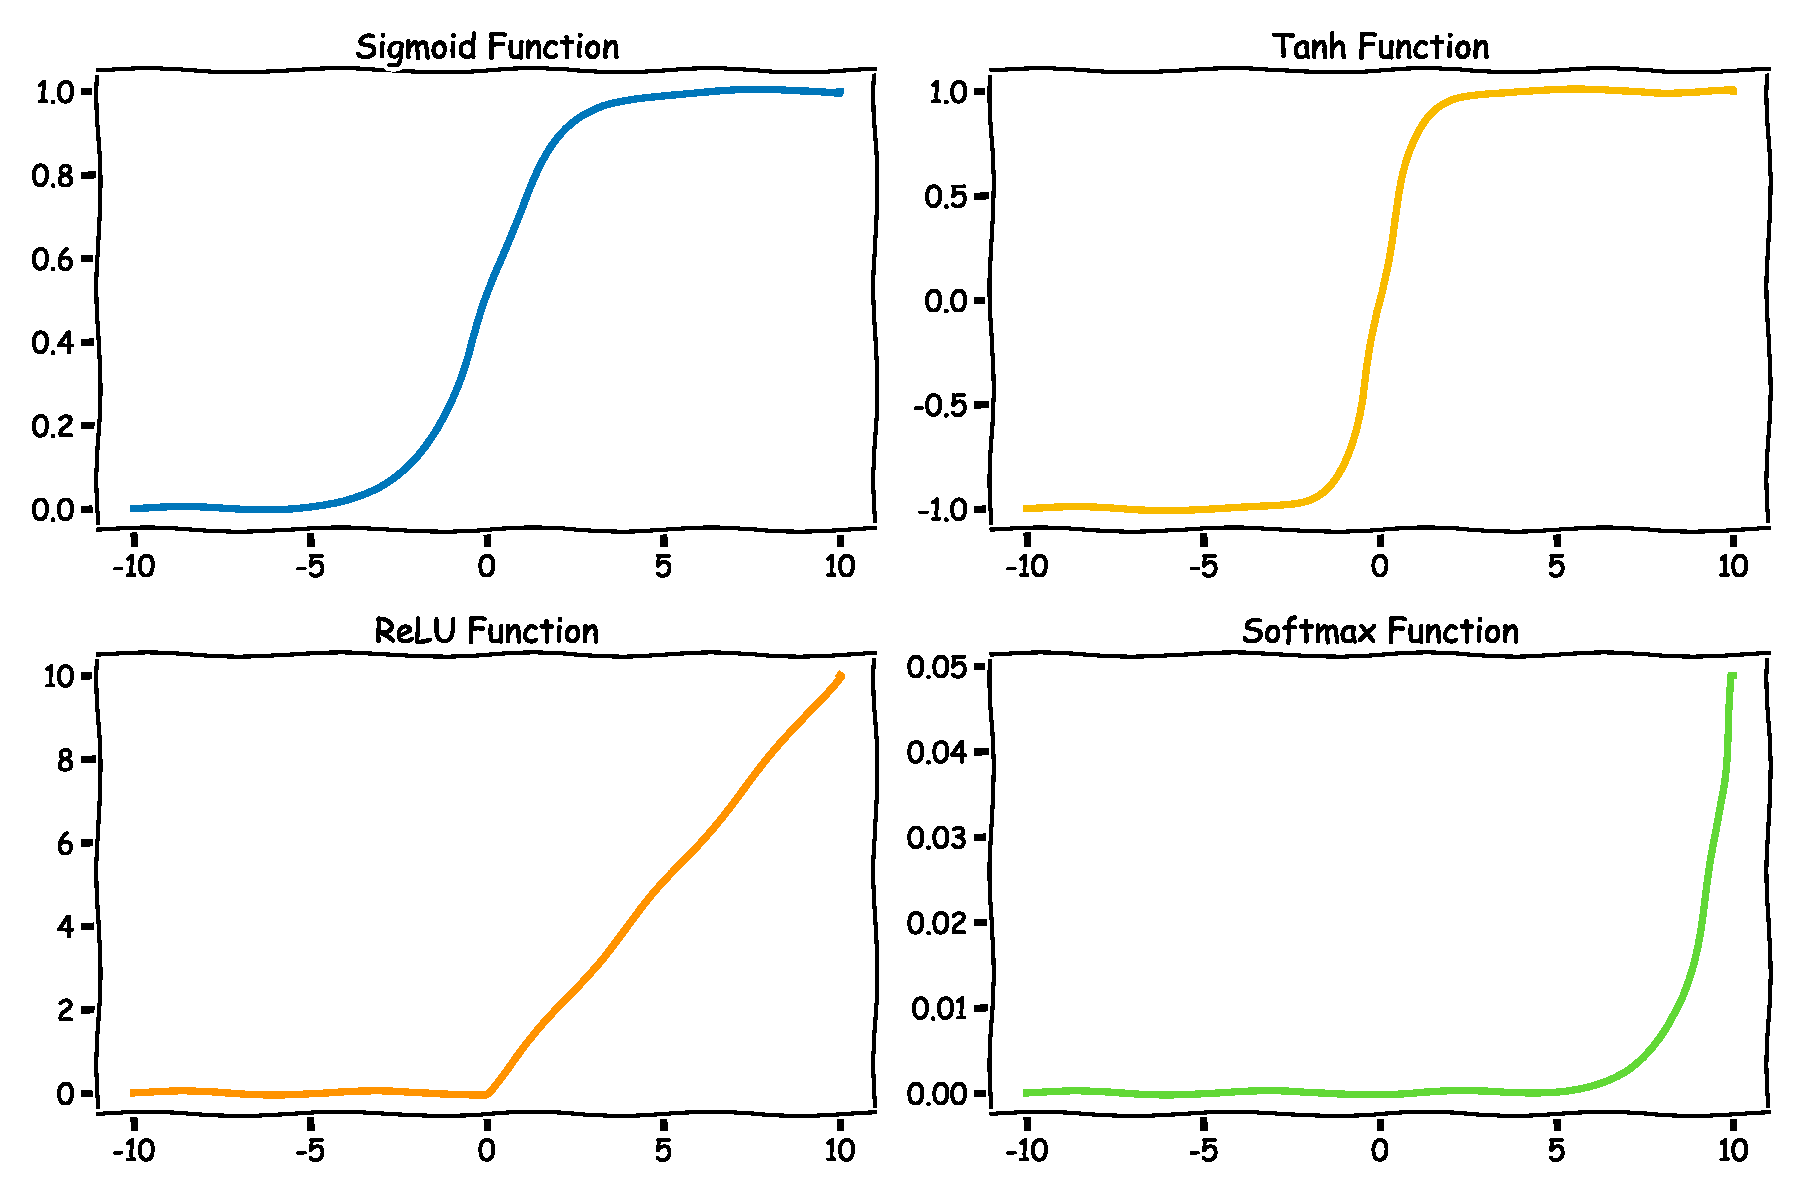
\includegraphics[width=1\linewidth]{LateX//figs/activation_functions_xkcd.pdf}
    \caption{Enter Caption}
    \label{fig:enter-label}
\end{figure}

ReLU (Rectified Linear Unit) is popular because it introduces non-linearity without saturating for positive values. Its derivative is:
% ReLU Derivative
\begin{equation}
    f'(\textit{net}_i) =
    \begin{cases}
    1, & \textit{net}_i > 0 \\
    0, & \textit{net}_i \leq 0
    \end{cases}
\end{equation}

This simplicity allows efficient back-propagation, enhancing computational speed during training.

\subsection{Neural Network Architecture}
Neural networks are generally organized in layers:
\begin{itemize}
    \item Input Layer: Takes in the raw data features.
    \item Output Layer: Outputs the final predictions.
    \item Hidden Layers: Contain intermediate neurons that extract hierarchical features. The presence of multiple hidden layers makes the network "deep," giving rise to deep neural networks (DNNs).
\end{itemize}

\begin{figure}
    \centering
    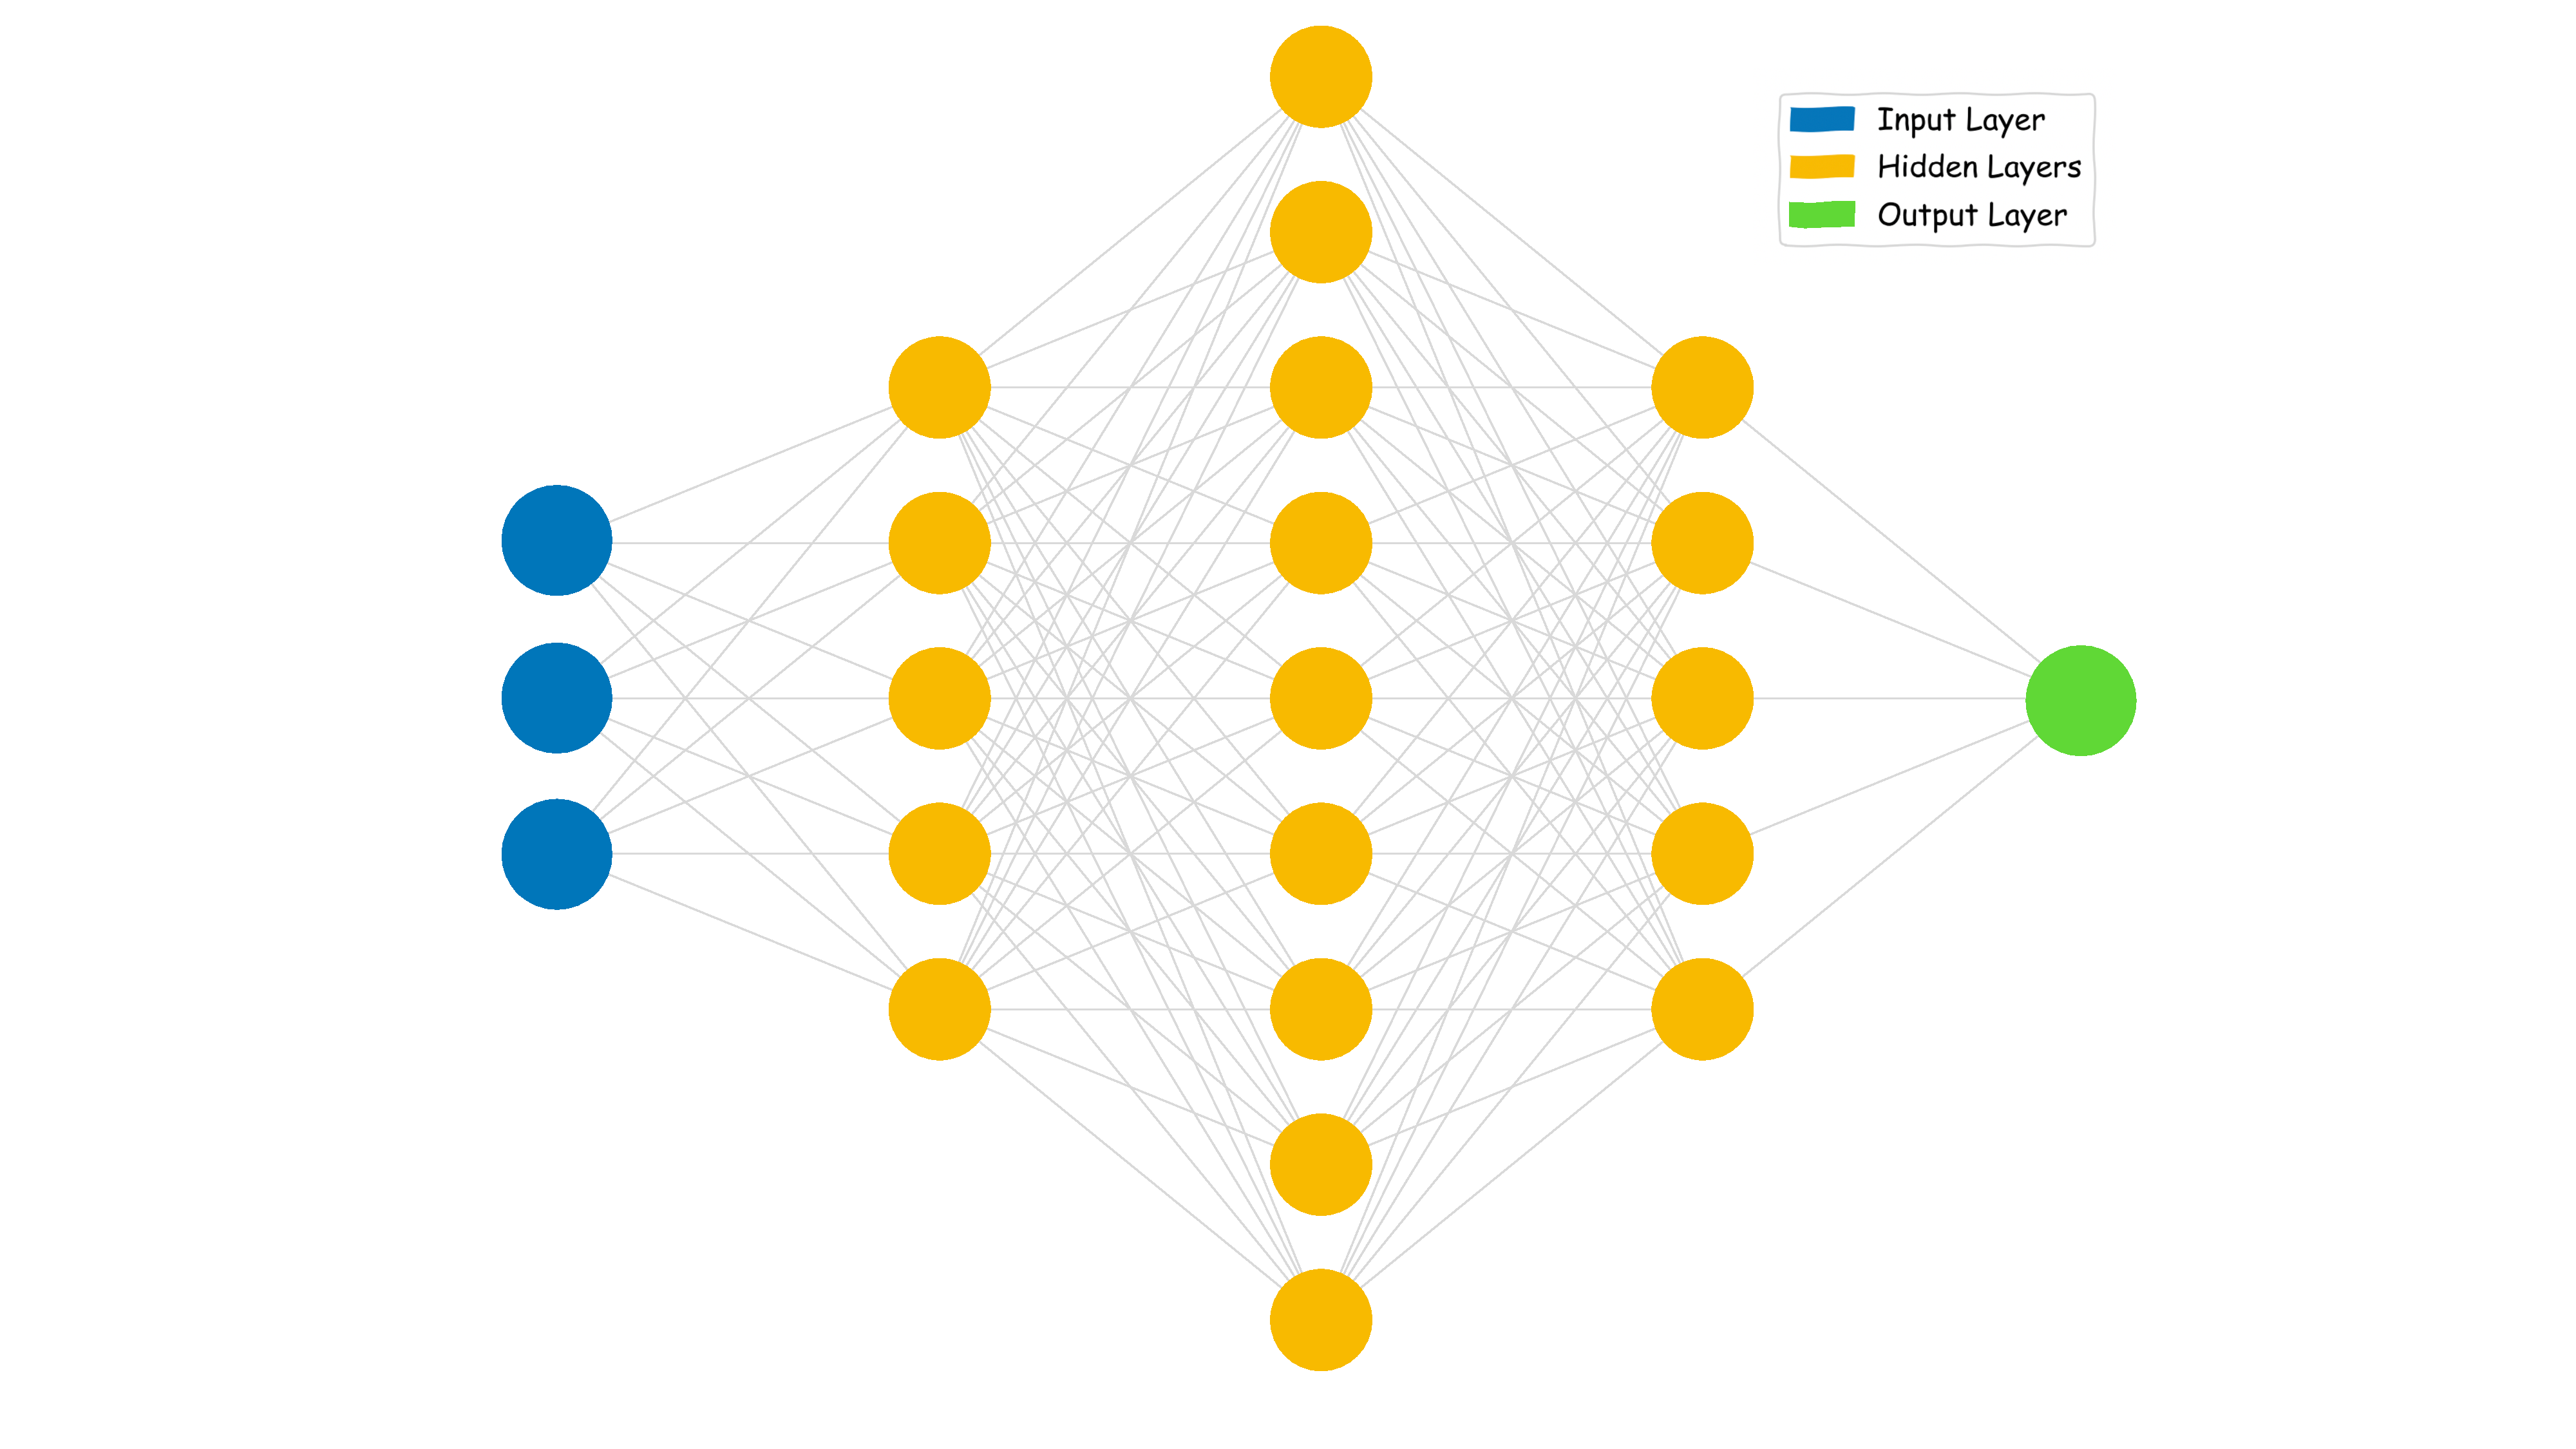
\includegraphics[width=0.9\linewidth]{LateX//figs/nn_intro_def.pdf}
    \caption{Enter Caption}
    \label{fig:enter-label}
\end{figure}

Forward Propagation
Once the network architecture is defined, information propagates from the input layer to the output layer in a process called forward propagation. This involves feeding inputs through each layer, applying the weights, summing them, and computing outputs using activation functions. The forward pass determines the final output for a given input.
Training Neural Networks
The goal of training a neural network is to find the optimal set of weights wji that map inputs to desired outputs. This process involves minimizing the difference between the network’s predictions and the actual targets, as measured by a loss function.
One of the most common loss functions is the sum of squared errors (SSE), given by:
% Sum of Squared Errors (SSE) Loss Function
\begin{equation}
    E(\mathbf{w}, \mathbf{x}) = \frac{1}{2} \sum_{i=1}^{N} (y_i - \hat{y}_i)^2
\end{equation}
where $y_i$ is the true label, $\hat{y}_i$ is the predicted output, and $N$ is the number of data samples.

\subsection{Gradient Descent and Back-propagation}
To minimize the loss function, neural networks use the gradient descent algorithm, which updates the weights by moving them in the direction opposite to the gradient of the loss function. The gradient represents the direction of the steepest increase in error, so stepping in the opposite direction reduces the error. The update rule is:
% Weight Update Rule Using Gradient Descent
\begin{equation}
    w_{ji} = w_{ji} - \eta \frac{\partial E}{\partial w_{ji}}
\end{equation}
Here, $\eta$ is the learning rate, a hyperparameter that controls the step size of the weight update. If the learning rate is too large, the network may not converge; if it’s too small, convergence will be slow. The backpropagation algorithm computes these gradients efficiently using the chain rule of calculus.
Stochastic Gradient Descent (SGD)
A more practical variant of gradient descent, especially for large datasets, is stochastic gradient descent (SGD). Instead of calculating the gradient for the entire dataset at once, SGD updates weights after each mini-batch of data points. This introduces randomness but speeds up training and often leads to better generalization.

\begin{algorithm}
\caption{Stochastic Gradient Descent (SGD)}
\begin{algorithmic}[1]
\State \textbf{Initialize:} weights $W_{ih}, W_{ho}, \eta$, batch size $B$, max epochs $T_{max}$
\State $t \gets 0$

\Repeat
    \State $t \gets t + 1$
    \State $L \gets 0$ \Comment{Initialize loss}
    \State Randomly shuffle the training set $\mathcal{D}$

    \For {each mini-batch $\mathcal{B}$ of size $B$}
        \State Reset gradient: $\nabla W_{ih} \gets 0, \nabla W_{ho} \gets 0$
        
        \For {each sample $x_i$ in $\mathcal{B}$}
            \State \textbf{Forward step:} $y_i \gets \text{forward}(x_i, W_{ih}, W_{ho})$
            \State Compute loss $L \gets L + \mathcal{L}(y_i, t_i)$
            
            \State \textbf{Backward step:} Compute gradients $\nabla W_{ho}, \nabla W_{ih}$ using backpropagation
        \EndFor

        \State Update hidden-output weights: $W_{ho} \gets W_{ho} - \eta \cdot \nabla W_{ho}$
        \State Update input-hidden weights: $W_{ih} \gets W_{ih} - \eta \cdot \nabla W_{ih}$
        
        \State $L \gets L / B$ \Comment{Average the loss}
    \EndFor
    
    \State Compute accuracy on the Train and Validation sets

\Until {(not convergence \textbf{and} $t < T_{max}$)}

\end{algorithmic}
\end{algorithm}

Learning Rate, Weight Decay, and Momentum
Several techniques help improve convergence:
    • Learning Rate: The learning rate $\eta$ controls how quickly weights are updated. It is crucial to select an appropriate value, as too large a rate can cause instability, while too small a rate can make training slow.
    • Weight Decay: This technique adds a regularization term to the loss function to prevent overfitting by penalizing large weight values. The modified loss function becomes:
% Weight Decay
\begin{equation}
    E(\mathbf{w}, \mathbf{x}) = \frac{1}{2} \sum_{i=1}^{N} (y_i - \hat{y}_i)^2 + \lambda \sum_{j=1}^{d} w_j^2
\end{equation}
where $\lambda$ is the regularization parameter.
    • Momentum: To speed up convergence and avoid getting stuck in local minima, momentum introduces a term that accumulates the gradient from previous updates:
% Momentum Update Rule
\begin{equation}
    v_t = \alpha v_{t-1} - \eta \frac{\partial E}{\partial w}
\end{equation}
where α is the momentum coefficient. This method helps smooth out oscillations in the weight updates.
Loss Functions
The choice of loss function depends on the task:
    • Mean Squared Error (MSE): Commonly used for regression tasks.
    • Cross-Entropy Loss: Often used for classification tasks. It compares the predicted probability distribution with the actual distribution of class labels.
Convergence and Generalization
During training, convergence is monitored by observing the loss function. If the loss decreases steadily and accuracy increases, the network is converging. Overfitting occurs when the model performs well on the training set but poorly on unseen data, indicating that the model has memorized the training data instead of generalizing. Techniques such as early stopping, regularization, and cross-validation help prevent overfitting.
The final goal of a neural network is to generalize well to unseen data, maximizing accuracy on both the training and validation sets. Careful tuning of hyperparameters and monitoring of the learning process ensures that the model learns effectively without over-fitting.

\subsection{Conclusion}
COPIARE QUI IMMAGINE 4 DEL PAPER \cite{10.11648/j.ajnna.20190501.12} (si trova alla pagina 10).

\begin{enumerate}
    \item Assign random weights to all the linkages to start the algorithm.
    \item Using the inputs and the (Input $\rightarrow$ Hidden Nodes) linkages, find the activation rate of Hidden Nodes.
    \item Using the activation rate of Hidden Nodes and linkages to Output, find the activation rate of Output Nodes.
    \item Find the error rate at the output node and re-calibrate all the linkages between Hidden Nodes and Output Nodes.
    \item Using the weights and error found at the Output node, cascade down the error to Hidden Nodes.
    \item Re-calibrate the weights between Hidden Nodes and Input Nodes.
    \item Repeat the process until the convergence criterion is met.
    \item Using the final linkage weights, score the activation rate of the Output Nodes.
\end{enumerate}




\section{Dataset}
Descrivere qui come è composto il dataset, devo dire che ci sono diverse sequenze che sono state registrate in diverse zone della città. per ogni frame (immagine) ci sono associati anche i dati che arrivano dal superdag. forse sul sito di ambarella si riesce a trovare qualche informazione sul superdag e sul suo funziomento. 
Il tutto viene impacchettato in un file .bin per gestire al meglio lo spazio. 
I dati vengono raccolti tramite alcune delle auto su cui VISLAB/Ambarella stanno sviluppando il loro sistema di guida autonoma. 
Ogni auto possiede una diversa sensor suite, che in generale è fornita da:
- front cameras
short cameras 
radars 
gps-gnsss che permette di localizzarsi nel mondo

\subsection{Sensor Suite}

\begin{figure}
    \centering
    \includegraphics[width=1\linewidth]{LateX//figs/sensor_suite2.pdf}
    \caption{Enter Caption. ci sono due cose da correggere, la prima è che in BEV cnon ci deve essere il radar centrale dietro, la seocnda è che in rear view c'è RR che non è centrato}
    \label{fig:enter-label}
\end{figure}


Descrivere qui le camere, magari aggiungere giusto qualche informazione sugli angoli di apertura ecc, anche qualche informazione sui radar e si potrebbe pensare di aggiungere quel grafico che era presente nelle slide in cui si vanno a vedere quelli che sono i pro e i contro delle svariate tecnologie. 

alla fine si mostra quindi quello che viene creato -> coppia, immagine e dati provenienti dal superdag. 
dire che cosa è il superdag: 




A DAG is a Directed Acyclic Graph, a type of graph whose nodes are directionally related to each other and don’t form a directional closed loop. In the practice of analytics engineering, DAGs are often used to visually represent the relationships between your data models.

While the concept of a DAG originated in mathematics and gained popularity in computational work, DAGs have found a home in the modern data world. They offer a great way to visualize data pipelines and lineage, and they offer an easy way to understand dependencies between data models.

In questo caso, sono collegati tutti i dati che provengono dallo stesso frame, in questo modo si riesce facilmente a vedere quali sono gli otuput sincronizzati di tutti i sensori. Le latenze dei diversi sensori, in questo modo, appaiono invisibili all'utente finale che si ritrova con un pacchetto di dati già sincronizzato. 


The Cflow processor is a hardware co-processor specially designed to execute
DAG representations of computer vision / Al algorithms.
• Directed acyclic graph (DAG) is a directed graph with no directed cycles. It consists of vertices and edges, with each edge directed from one vertex to another, such that following those directions will never form a closed loop.
• Nodes in the graph represent the computational operations and links represent the flow of data between them.
• Data is represented as multi-dimensional tensors:
• Image is 2D vector.
• No pointer, direct memory access, ....
• Operations are performed in parallel by available hardware resources (datapath):
E
• Multiple instruction, multiple data architecture (MIMD).
• Custom operations.

https://hazelcast.com/glossary/directed-acyclic-graph/
https://medium.com/@danthelion/core-data-engineering-dags-36ce241b32d5
\begin{figure}
    \centering
    \includegraphics[width=1\linewidth]{LateX//figs/loss_functions_xkcd.pdf}
    \caption{Enter Caption}
\begin{figure}
        \centering
        \includegraphics[width=1\linewidth]{LateX//figs/loss_functions_xkcd.pdf}
        \caption{Enter Caption}
        \label{fig:enter-label}
    \end{figure}
        \label{fig:enter-label}
\end{figure}
questo è altro che si è trovato sulle slide riguardo a quello. 

Specificare quindi tutto quel che trovo riguardo a SuperDAG, cvflow ecc usando le pagine ambarella come fonte sicura. Guardare anche quelle slide che ci sono sul pc, magari possono essere utili. 

creare una rappresentazione 


---
giunti al termine, parlare delle vie della città in cui le sequenze che possiedo sono state registrate, fare un calcolo dei frame e parlare della divisione del dataaset tra parte di training e parte di validation. Parlare anche che, nel corso dello svilupoo del progetto, sono stati utilizzati due split diversi, per iniziare uno che utilizzava solo sequenze di una determinata zona (in modo da avere meno dapi e concentrarsi sulla struttura) e successivamente, una volta chiusa la quadra e trovato il modo giusto di lavorare, si è deciso di ampliare con tutte le sequenze registrate ottenute. 








\subsection{Preprocessing}
The BEVPreprocessor class is designed to perform preprocessing operations on inputs before passing them to the main model in a bird's-eye-view (BEV) perception pipeline. This preprocessor is particularly tailored for scenarios where multiple input features need to be aggregated and transformed into a unified format. Below is a detailed analysis of each section of the code.

Initialization:

The constructor $(__init__)$ initializes the BEVPreprocessor by accepting two arguments:

cfg: A configuration object (CfgNode) that holds the settings for the dataset, including whether ego-related data should be included.
$in_channels$: A dictionary that maps input feature names to their respective channel dimensions.
During initialization, it retrieves the setting for EGO from the dataset configuration and sets up a 1x1 convolutional layer (conv1x1) to perform a channel transformation. This convolutional layer takes in an input tensor with 34 channels and outputs a tensor with 38 channels, adapting the input features to match the expected size for subsequent stages of the network.

Forward Method:
The forward function processes the input features, concatenates them along the channel dimension, and applies a transformation via the convolutional layer. The function:

Takes a dictionary of input tensors as an argument, with keys corresponding to different types of input features.
Accumulates the relevant feature maps ($cam2bev_feats$, rgb2bev, observations, topology, regulations, ego) into a list.
The ego feature is only included if it is present in the input and the EGO flag is set to True in the configuration. The unsqueeze operation on the ego feature adjusts its dimensionality for concatenation.
These features are concatenated along the channel dimension (i.e., the third dimension, indexed as -3).
Finally, a 1x1 convolutional layer is applied to the concatenated tensor to produce the output with the desired number of channels.
The method returns two values:

x: The transformed tensor after concatenation and convolution.
An empty dictionary {} as a placeholder for any additional outputs that may be required in future implementations.
This preprocessing step ensures that input features from various modalities are efficiently combined and reshaped, allowing the main model to work with a consistent representation. The use of 1x1 convolution reduces computational complexity while enabling flexible channel transformations.

\begin{algorithm}[H]
\caption{BEVPreprocessor Forward Pass}
\SetKwInOut{Input}{Input}
\SetKwInOut{Output}{Output}

\Input{Input features dictionary \texttt{input}, Configuration object \texttt{cfg}}
\Output{Transformed tensor $x$, Optional outputs dictionary}

\BlankLine
\textbf{Initialize:} 
\begin{itemize}
  \item \texttt{ego} flag from configuration \texttt{cfg.DATASET.INPUT.EGO}
  \item 1x1 Convolution layer \texttt{conv1x1}, with 34 input channels and 38 output channels
\end{itemize}

\BlankLine
\textbf{Forward Pass:}

1. Create an empty list $x$

2. \ForEach{feature in \texttt{input} dictionary}{
   Append feature to $x$ if available, from:
   \begin{itemize}
       \item \texttt{cam2bev\_feats}
       \item \texttt{rgb2bev}
       \item \texttt{observations}
       \item \texttt{topology}
       \item \texttt{regulations}
       \item \texttt{ego} (only if \texttt{ego} flag is True, after adding an additional channel dimension)
   \end{itemize}
}

3. Concatenate all features in $x$ along the channel dimension (-3)

4. Apply 1x1 convolution: $x = \texttt{conv1x1}(x)$

\BlankLine
\Return{$x$, \{\}}

\end{algorithm}


\begin{verbatim}
# Preprocessor configuration
preprocessor_config = {
    'name': 'BEVPreprocessor',
    'normalize_output': False,
    'grid_sample_mode': ['bilinear'],
    'locnet_backbone_channels': [32, 64, 128, 256, 256]
}
\end{verbatim}

Qui viene riportato direttamente il codice del preprocessore, in modo che si possa andare a capire esattamente quello che succede. 


The following pseudocode outlines the structure and operations of a Bird’s Eye View (BEV) preprocessor used in autonomous driving systems. The preprocessor integrates different types of sensor inputs (e.g., camera, RGB, topology, and regulations) and combines them into a unified format for further processing. A key feature of this preprocessor is the use of a 1x1 convolution to adjust the number of input channels, which optimizes the data for subsequent layers in a neural network.

\begin{algorithm}
\caption{BEV Preprocessor Forward Pass}
\begin{algorithmic}[1]
\State \textbf{Input:} Configuration $cfg$, Input Channels $in\_channels$, Input Tensors $input$
\State \textbf{Output:} Transformed Tensor $y$, Optional Outputs $out$

\State \textbf{Initialize:} 
\State \hspace{1cm} $ego \gets cfg.DATASET.INPUT.EGO$
\State \hspace{1cm} $conv1x1 \gets \text{Conv2d}(in\_channels=34, out\_channels=38, kernel\_size=1)$
\State $x \gets []$ \Comment{Initialize empty list to store features}

\If{'cam2bev\_feats' in input}
    \State Append $input['cam2bev\_feats']$ to $x$
\EndIf
\If{'rgb2bev' in input}
    \State Append $input['rgb2bev']$ to $x$
\EndIf
\If{'observations' in input}
    \State Append $input['observations']$ to $x$
\EndIf
\If{'topology' in input}
    \State Append $input['topology']$ to $x$
\EndIf
\If{'regulations' in input}
    \State Append $input['regulations']$ to $x$
\EndIf
\If{'ego' in input \textbf{and} $ego = \text{True}$}
    \State Append $input['ego'].unsqueeze(-3)$ to $x$
\EndIf

\State $x \gets \text{Concatenate}(x, dim=-3)$ \Comment{Concatenate features along the channel dimension}
\State $y \gets conv1x1(x)$ \Comment{Transform channel dimensions with 1x1 convolution}

\State \Return $y, \{\}$ \Comment{Return transformed tensor and an empty dictionary}
\end{algorithmic}
\end{algorithm}


\begin{figure}
        \centering
        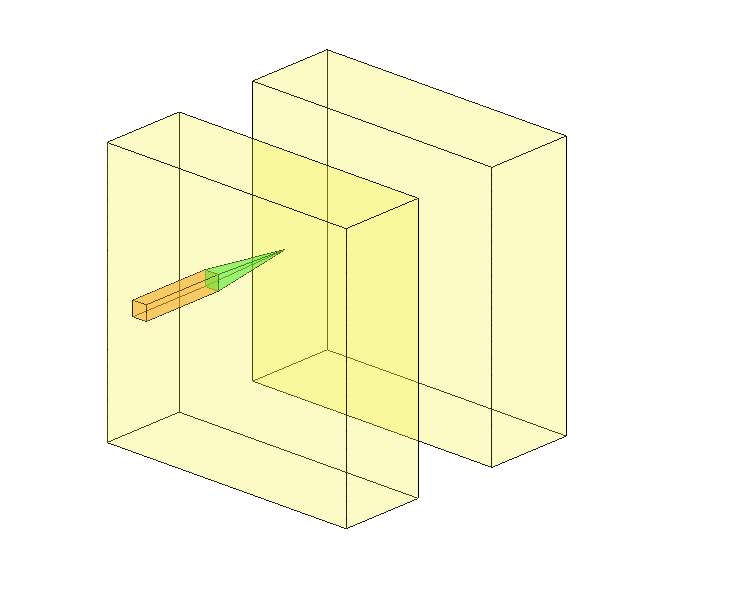
\includegraphics[width=0.75\linewidth]{LateX//figs/download.png}
        \caption{Enter Caption}
        \label{fig:enter-label}
\end{figure}






\begin{verbatim}





@PREPROC_REGISTRY.register()
class BEVPreprocessor(Preprocessor):

RICORDARSI CHE NEL MIO CONFIG QUEL DATASET EGO è FALSE, QUINDI TENERLO IN CONSIDERAZIONE

  # Initialize with configuration and input channels
  Initialize(cfg: CfgNode, in_channels: Dict[str, int]):
    - Set ego as cfg.DATASET.INPUT.EGO
    - Create conv1x1: Conv2d with 34 input channels and 38 output channels

  # Define the forward pass
  forward(input: Dict[str, Tensor]) -> Tuple[Tensor, Dict[str, Tensor]]:
    - Initialize empty list x
    - If 'cam2bev_feats' in input:
        Append 'cam2bev_feats' to x
    - If 'rgb2bev' in input:
        Append 'rgb2bev' to x
    - If 'observations' in input:
        Append 'observations' to x
    - If 'topology' in input:
        Append 'topology' to x
    - If 'regulations' in input:
        Append 'regulations' to x
    - If 'ego' in input and ego is enabled:
        Append 'ego' (with an additional dimension) to x

    - Concatenate x along the channel dimension (-3)
    - Apply conv1x1 to x

    - Return the transformed tensor and an empty dictionary
\end{verbatim}


\begin{verbatim}
    @PREPROC_REGISTRY.register()
class BEVPreprocessor(Preprocessor):
  def __init__(self, cfg: CfgNode, in_channels: Dict[str, int]):
    super().__init__(cfg, in_channels)

    self.ego = cfg.DATASET.INPUT.EGO
    self.conv1x1 = torch.nn.Conv2d(in_channels=34, out_channels=38, kernel_size=1)

  def forward(self, input: Dict[str, Tensor]) -> Tuple[Tensor, Dict[str, Tensor]]:
    """
    Args:
      input (Dict[str, Tensor]): tensors used to compute the transform.

    Returns:
      y   (Tensor)           : transformed input.
      out (Dict[str, Tensor]): optional outputs of the preprocessor.
    """
    x = []
    if 'cam2bev_feats' in input:
      x.append(input['cam2bev_feats'])
    if 'rgb2bev' in input:
      x.append(input['rgb2bev'])
    if 'observations' in input:
      x.append(input['observations'])
    if 'topology' in input:
      x.append(input['topology'])
    if 'regulations' in input:
      x.append(input['regulations'])
    if 'ego' in input and self.ego:
      x.append(input['ego'].unsqueeze(-3))
      
    x = torch.cat(x, dim=-3)
    x = self.conv1x1(x)  # transform the number of channels
    
    # print(x.shape, 'dimensioni di x alla fine del nuovo preoprocessor ')
    return x, {}
\end{verbatim}

\subsection{Input Loaders}
Qui per esempio potrei pensare di andare a definire tutti gli input loader che utilizzo, andando nel dettaglio di quelli più succosi o meglio quelli che mi interessano di più. 
Io pensavo di metterli tutti, sia quelli utilizzati nelle prime run, sia quelli che vengono utilizzati solamente più tardi nel processo. Sarà poi mia premura, quando spiegherò come è avvenuta la prima parte del progetto, dire che solo alcuni degli input loader sono stati utilizzati.

Parlare del fatto che la mappa viene rappresentata sull'immagine con una deterimanta precisione ecc. (si tratta di un pixel per 25cm)

# Size of the map area to query
_C.DATASET.MAP_SIZE = CN()
_C.DATASET.MAP_SIZE.XMIN = -32.0
_C.DATASET.MAP_SIZE.XMAX =  96.0
_C.DATASET.MAP_SIZE.YMIN = -32.0
_C.DATASET.MAP_SIZE.YMAX =  32.0
_C.DATASET.MAP_SIZE.CONTOUR = 50.0

_C.DATASET.MAP_COMPRESSION = CN()
# Map compression type - Options: 0 (no compression), 1 (linear), 2 (quadratic), ...
_C.DATASET.MAP_COMPRESSION.TYPE = 0
# Map px per m resolution in the non compressed area
_C.DATASET.MAP_COMPRESSION.X_STEP = 5.0
_C.DATASET.MAP_COMPRESSION.Y_STEP = 5.0
# Distance after which the map is compressed
_C.DATASET.MAP_COMPRESSION.X_DIST = 50.0
_C.DATASET.MAP_COMPRESSION.Y_DIST = 20.0

parlare anche delle dimensioni generali dela query (forse specificare anche di che cosa si tratta).

In the context of autonomous vehicle systems, the conversion of sensor data into a multi-channel tensor representation is critical for accurate environmental perception and decision-making. The sensors, such as LiDAR, radar, and cameras, capture real-time spatial and orientation data in the vehicle’s surrounding environment. This data is typically in a world-coordinate system, such as the East-North-Up (ENU) reference frame, and must be transformed into a structured format suitable for neural network processing. The conversion process involves mapping these spatial coordinates onto a 2D canvas, where each sensor’s output can be visualized on a dedicated channel of the tensor. This multi-channel tensor serves as the input to convolutional neural networks (CNNs), enabling the system to interpret the vehicle's surroundings with high precision. Key to this approach is the use of coordinate-to-canvas conversion techniques, which ensure the spatial data is accurately represented. Additionally, resampling methods are employed to create uniform and consistent point distributions, especially when dealing with data from multiple sensors with varying resolutions. By integrating sensor data in this manner, the system can effectively represent complex environmental features, such as object locations, trajectories, and orientations, enabling robust decision-making for tasks like obstacle detection, path planning, and motion prediction.

QUI SOPRA POTREBBE ESSERCI UN'INTRODUZIONE ALLA COSA, SAREBBE ANCHE CARINO FARE UNO PSUDOCODE CHE FA CAPIRE COME TUTTI GLI INOUT LAODER PER CREARE QUESTA IMMAGINE FANNO PARTE DI UNA STESSA CLASSE PADRE DI APPARTENENZA CHE RICHIEDE LORO DETERMINATE CARATTERISTICHE. 

Gli input loader(S) che ho usato sono:
- BEVObservationsLoader, EgoLoader, BoundariesInputLoader, TextureLoader, HorizontalFOVLoader, BEVWarpLoader, CamPosLoader, AttAugmentedCooordLoader, DirVectorLoader

partiamo dal

\subsubsection{BevObservationsLoader}

\begin{figure}
    \centering
    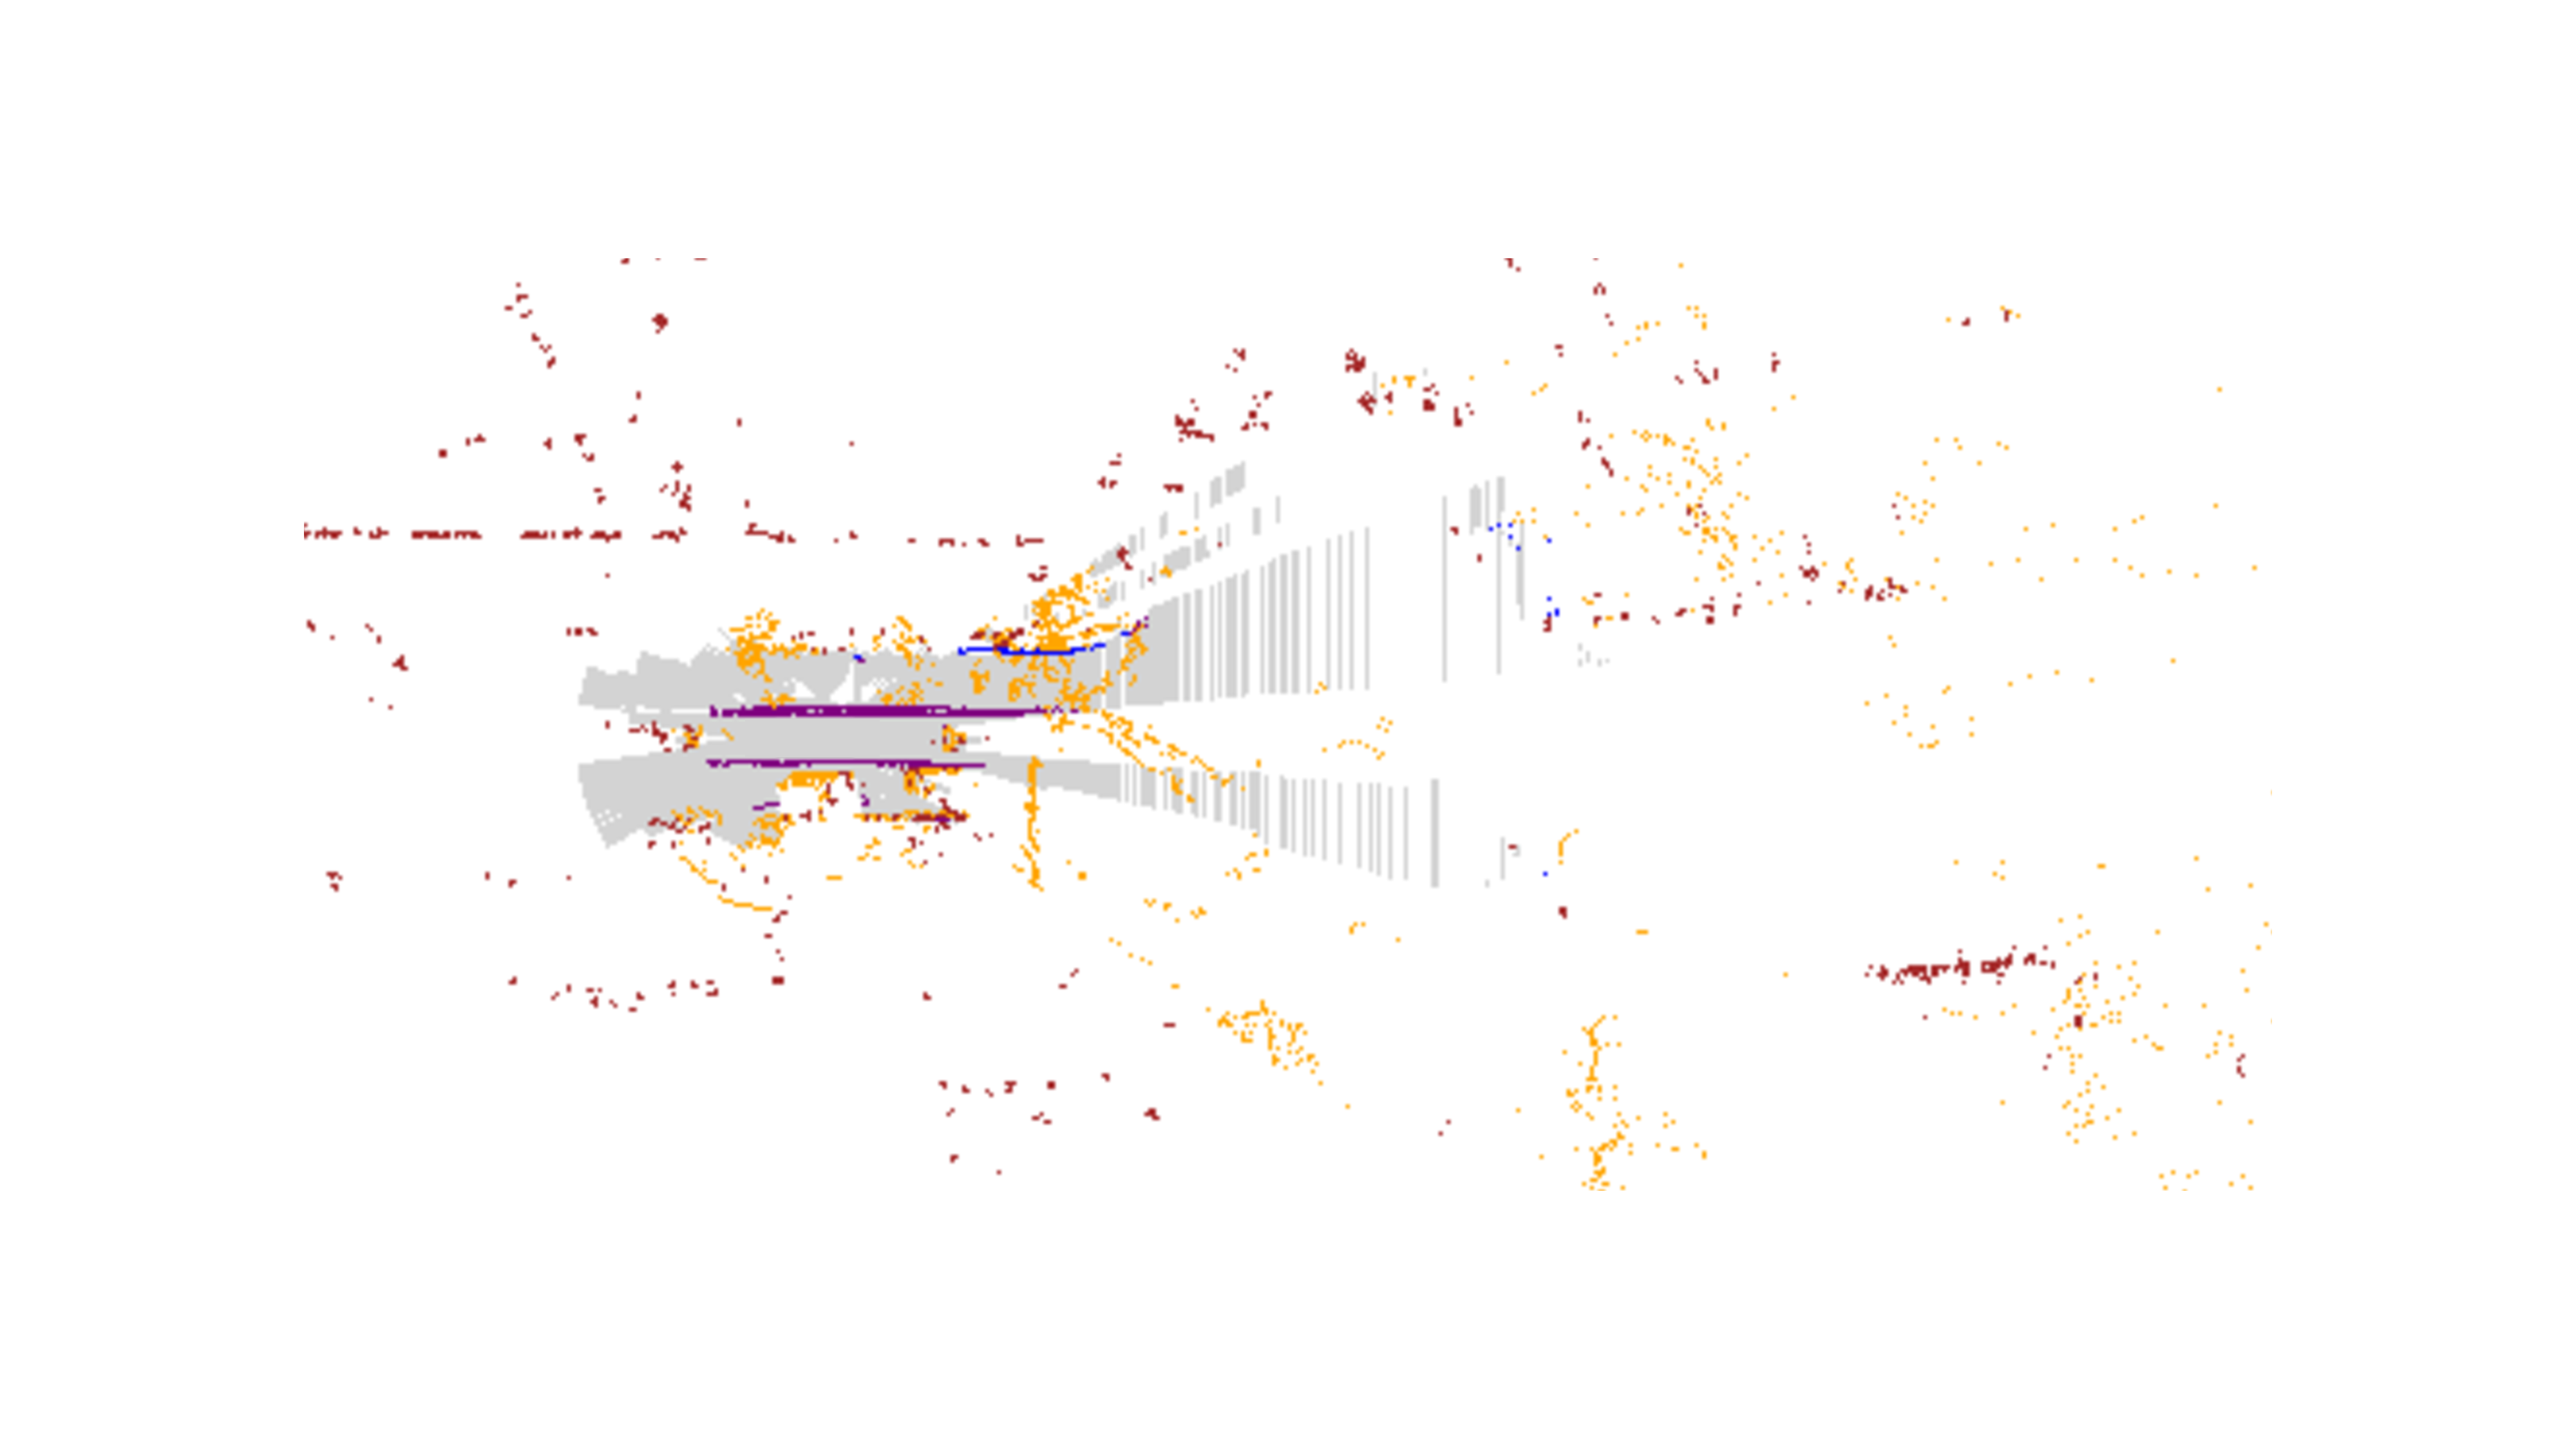
\includegraphics[width=1\linewidth]{LateX//figs/bevLoader.pdf}
    \caption{Enter Caption}
    \label{fig:enter-label}
\end{figure}

It creates a tensor representing all the BEV measures, It take all the data that comes from the serialization binary file and returna atrensor representing BEV measures divided between the following channels, lane markings, road boundaries, free spaces, traffic signs, obstacles, stixels, parking and instances a seconda di quello che è stato selezioanato nel file configuratore. 
A questo punto, le cose da fare, sono convertire le diverse tipologie di coordinate dei dati provienti dai diversi sensori, in coordinate immagine, in modo da andare a stmapare tutto sul tensore a più canali che va a rappresentare il tutto. 
Nel codice si trova che cosa viene fatto nello specifico per ogni dato, darci un'occhiata e riportare qui un riassunto. 
Per le immagini bisogna infatti effettuare determinate operazioni, per i radar altre ecc..

\subsubsection{EGOLoader}
Questa parte di codice va a rappresentare, nello stesso tensore che stiamo indagando, un 5x2 vehicle con le sue ego-measures. 
Viene chiamata una funzione che restituisce un rettangolo, e vengono passate le dimensioni del veicolo a seconda del quale è stato effettivamente utilizzato per registrare le sequenze del dataset, e anche le sue coordinate, tra cui i punti nello spazio e ele sue orientazioni (heading in particolar modo). 

\begin{figure}
    \centering
    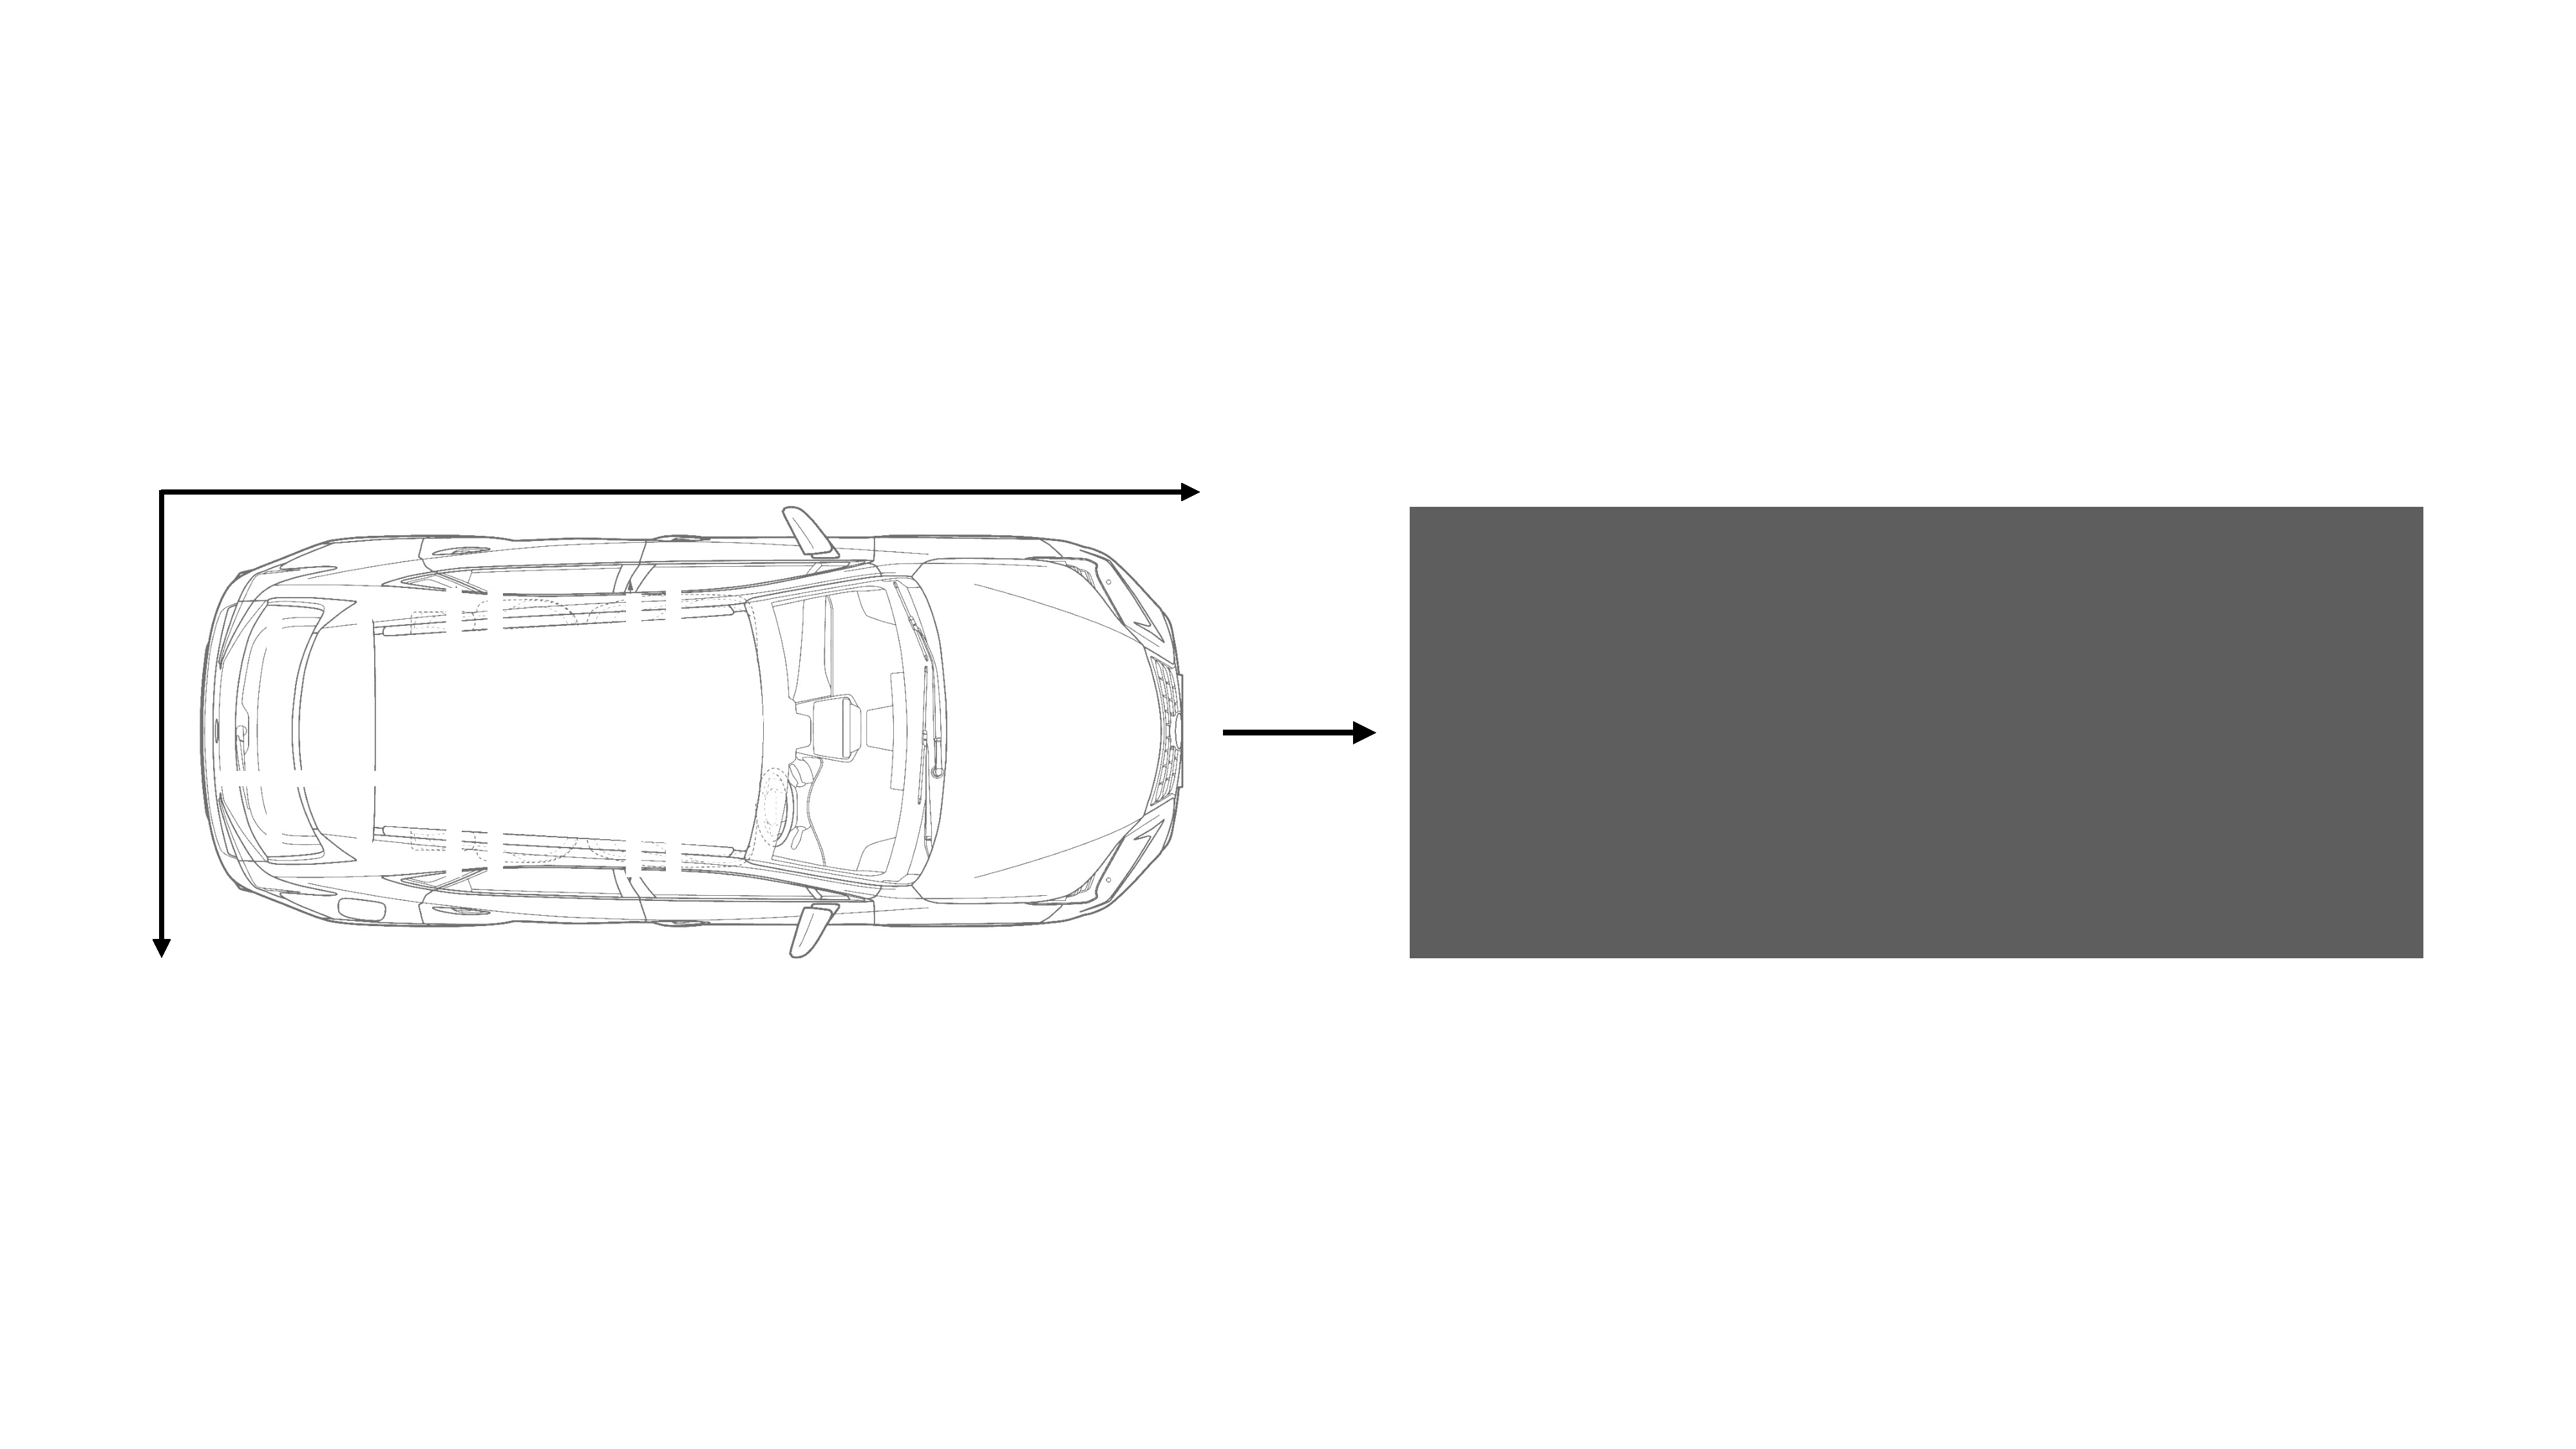
\includegraphics[width=0.75\linewidth]{LateX//figs/egoLoader.pdf}
    \caption{Enter Caption}
    \label{fig:enter-label}
\end{figure}

\subsubsection{BoundariesInputLoader}
Questo è tutta farina del mio sacco, in quanto prima questo si trovava nel target, nell'applicazione che la stessa rete aveva in precedenza (questa cosa non so neanche se valga la pena dirla, visto che in teoria dovrebbe passare come tutto alvoro mio). 
Questo input loader si occupa di semantic segmantation. Va a creare un tensore che rappresenta i boundaries e prende in ingresso un solito dizionario con al'interno i dati della mappa dell'area di riferimento. Parlare anche della dimensione del riferimento, che viene gestita sempre dal file di configurazione. Ci sono infatti dei limiti sia per quanto riguarda l'altezza sia per quanto riguarda la larghezza della zona di cui si va a scaricare la mappa rispetto alla posizione corrente del veicolo. 

Farsi spiegare esattamente il comportamente del codice, ma in linea di massa va a prendere i dati dalla mappa e li disegna. nella mapppa ci sono i boundaries che sono di varie categorie (magari mettere un'immagine di quelli che sono i boundaries). 
In autonomous driving, "boundaries" refer to the limits or edges of a vehicle's operational environment. These can include physical elements like the edges of a road, curbs, walls, or even virtual markers in a mapped area that define where the vehicle is allowed to operate. Boundaries are broader than lanes, which specifically define the designated space within a road where a vehicle is supposed to travel. While lanes guide a vehicle along a path of travel, boundaries prevent the vehicle from leaving its safe operating area or driving into restricted zones. Essentially, boundaries are concerned with keeping the vehicle within the permitted environment, while lanes focus on its alignment within the road.

\begin{figure}
    \centering
    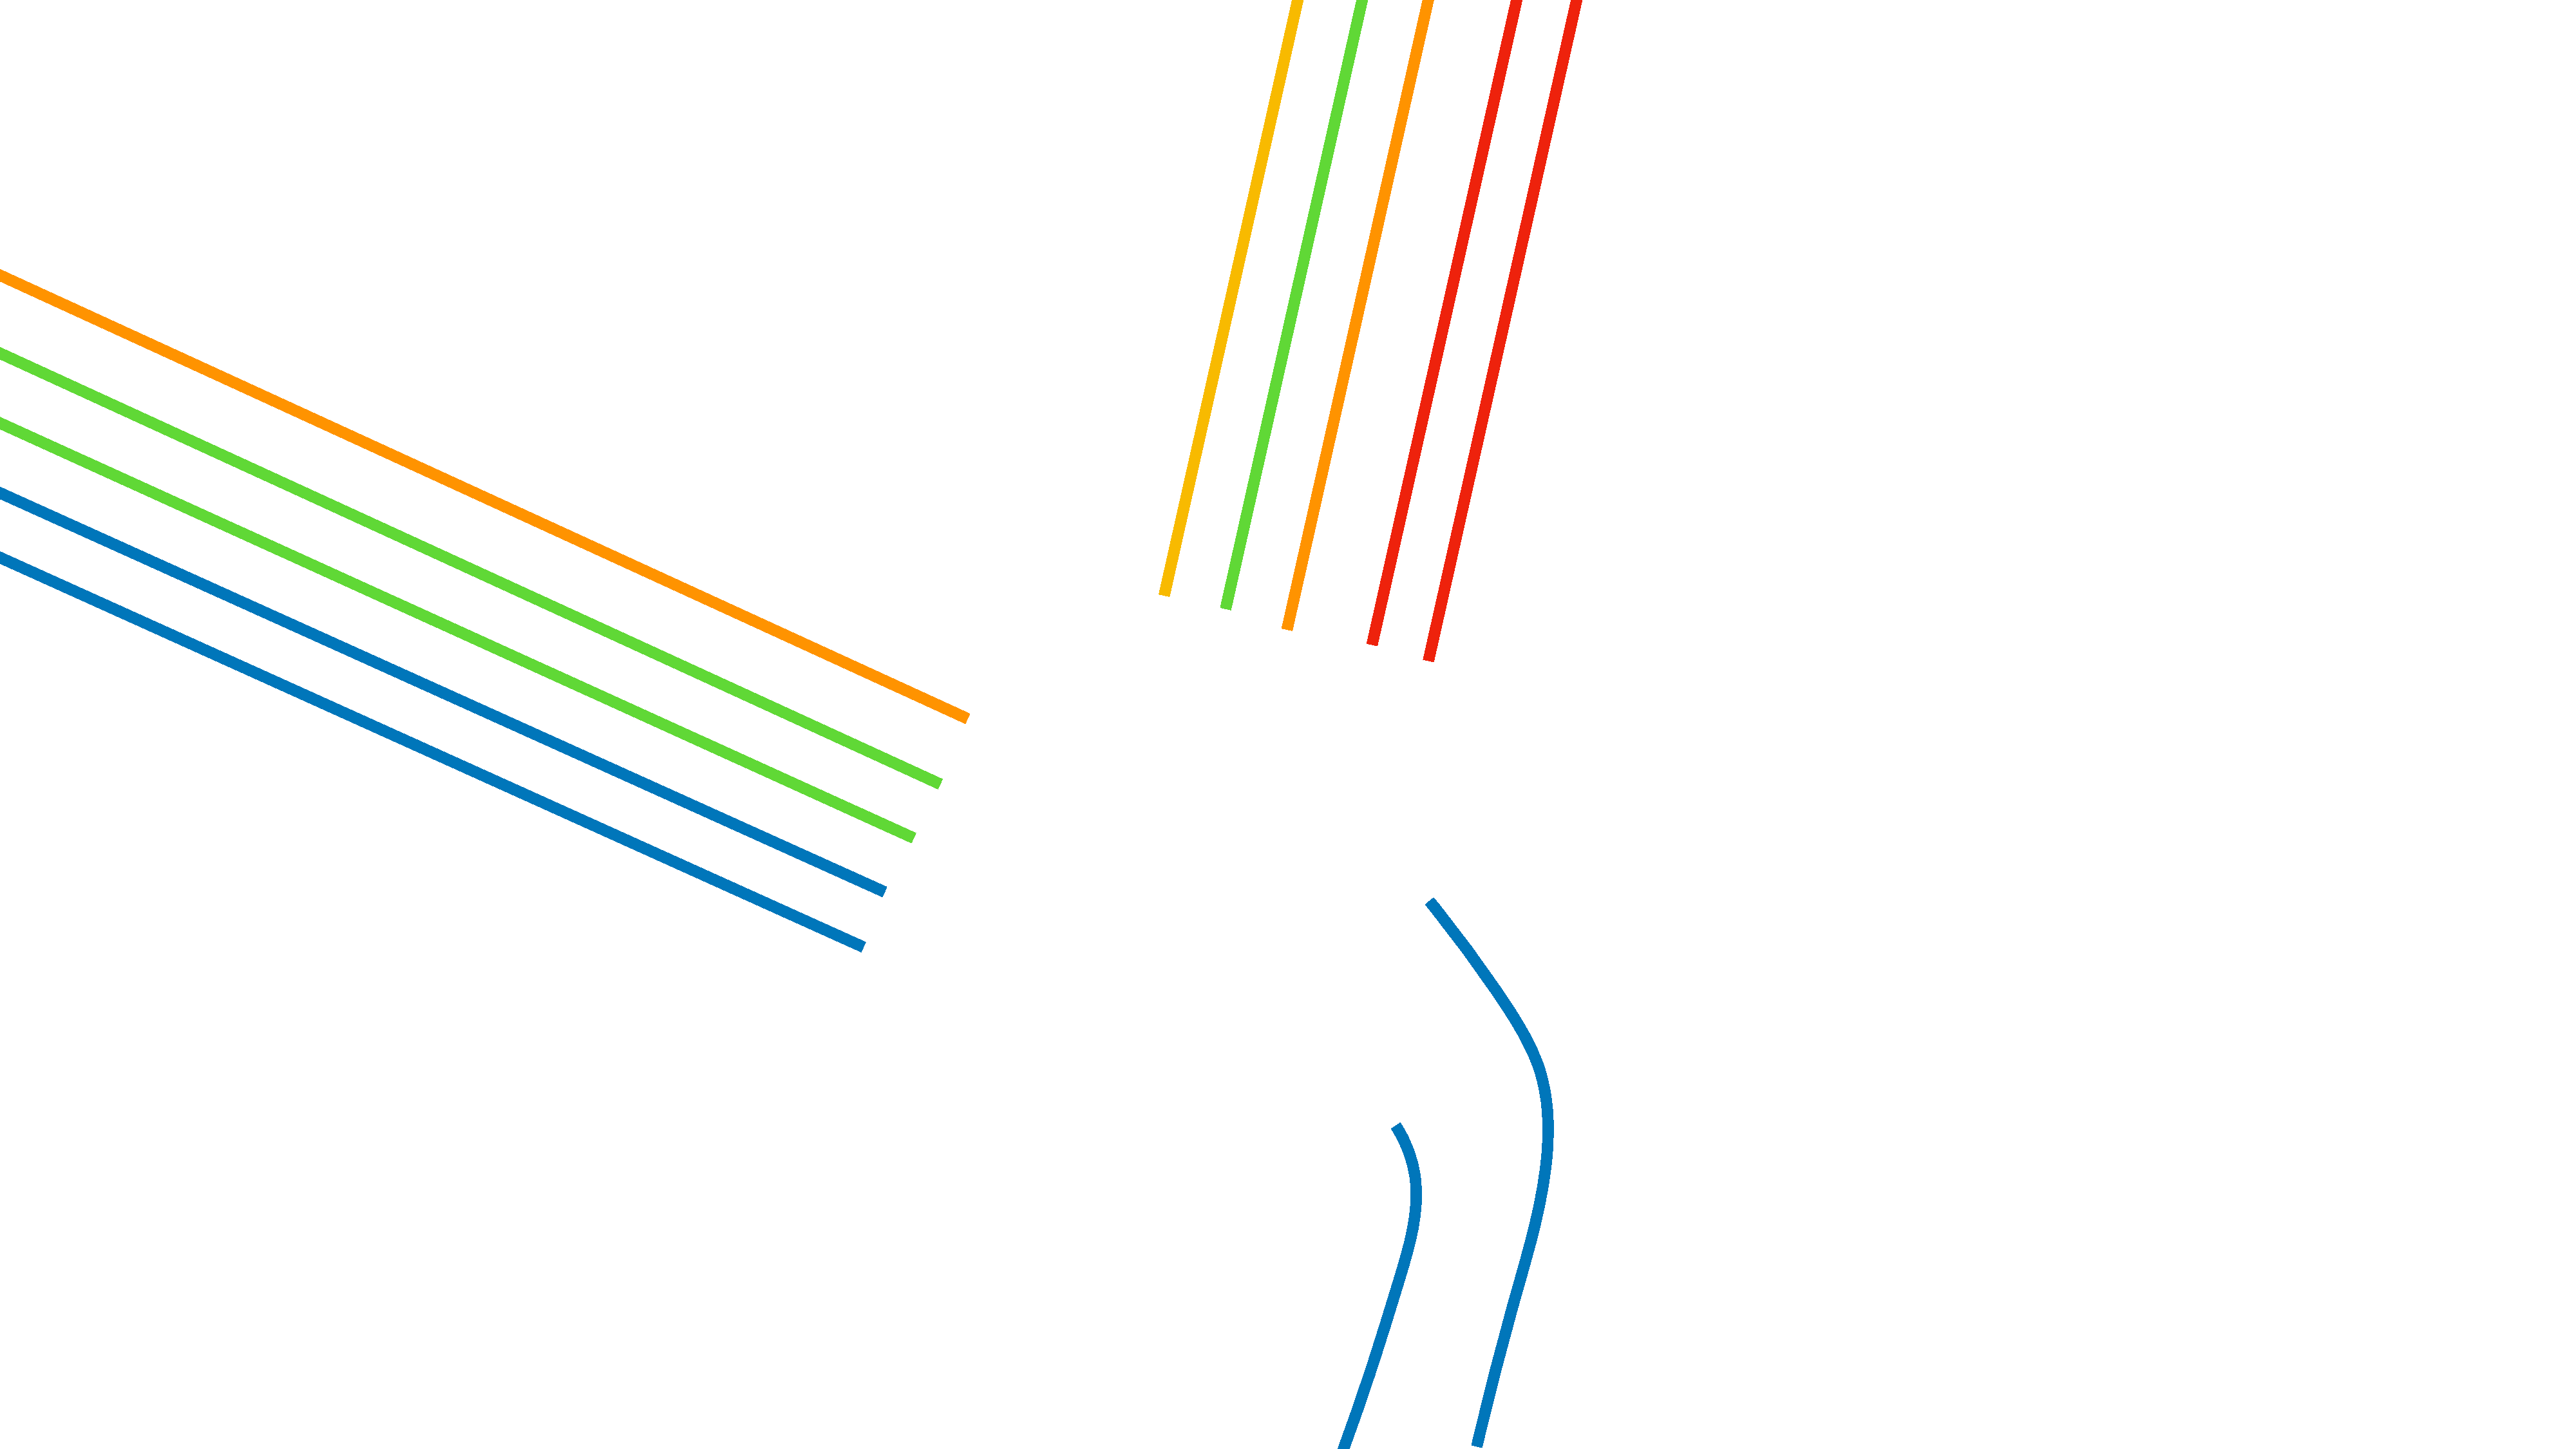
\includegraphics[width=0.75\linewidth]{LateX//figs/mappaHD.pdf}
    \caption{Enter Caption}
    \label{fig:enter-label}
\end{figure}

\subsubsection{TextureLoader}
Se non ricordo male, questo si occupa semplicemente di caricare tutte le immagini provienti dalle diverse camere viste nel paragrafo in cui parlo della sensors suite. 

\begin{figure}
    \centering
    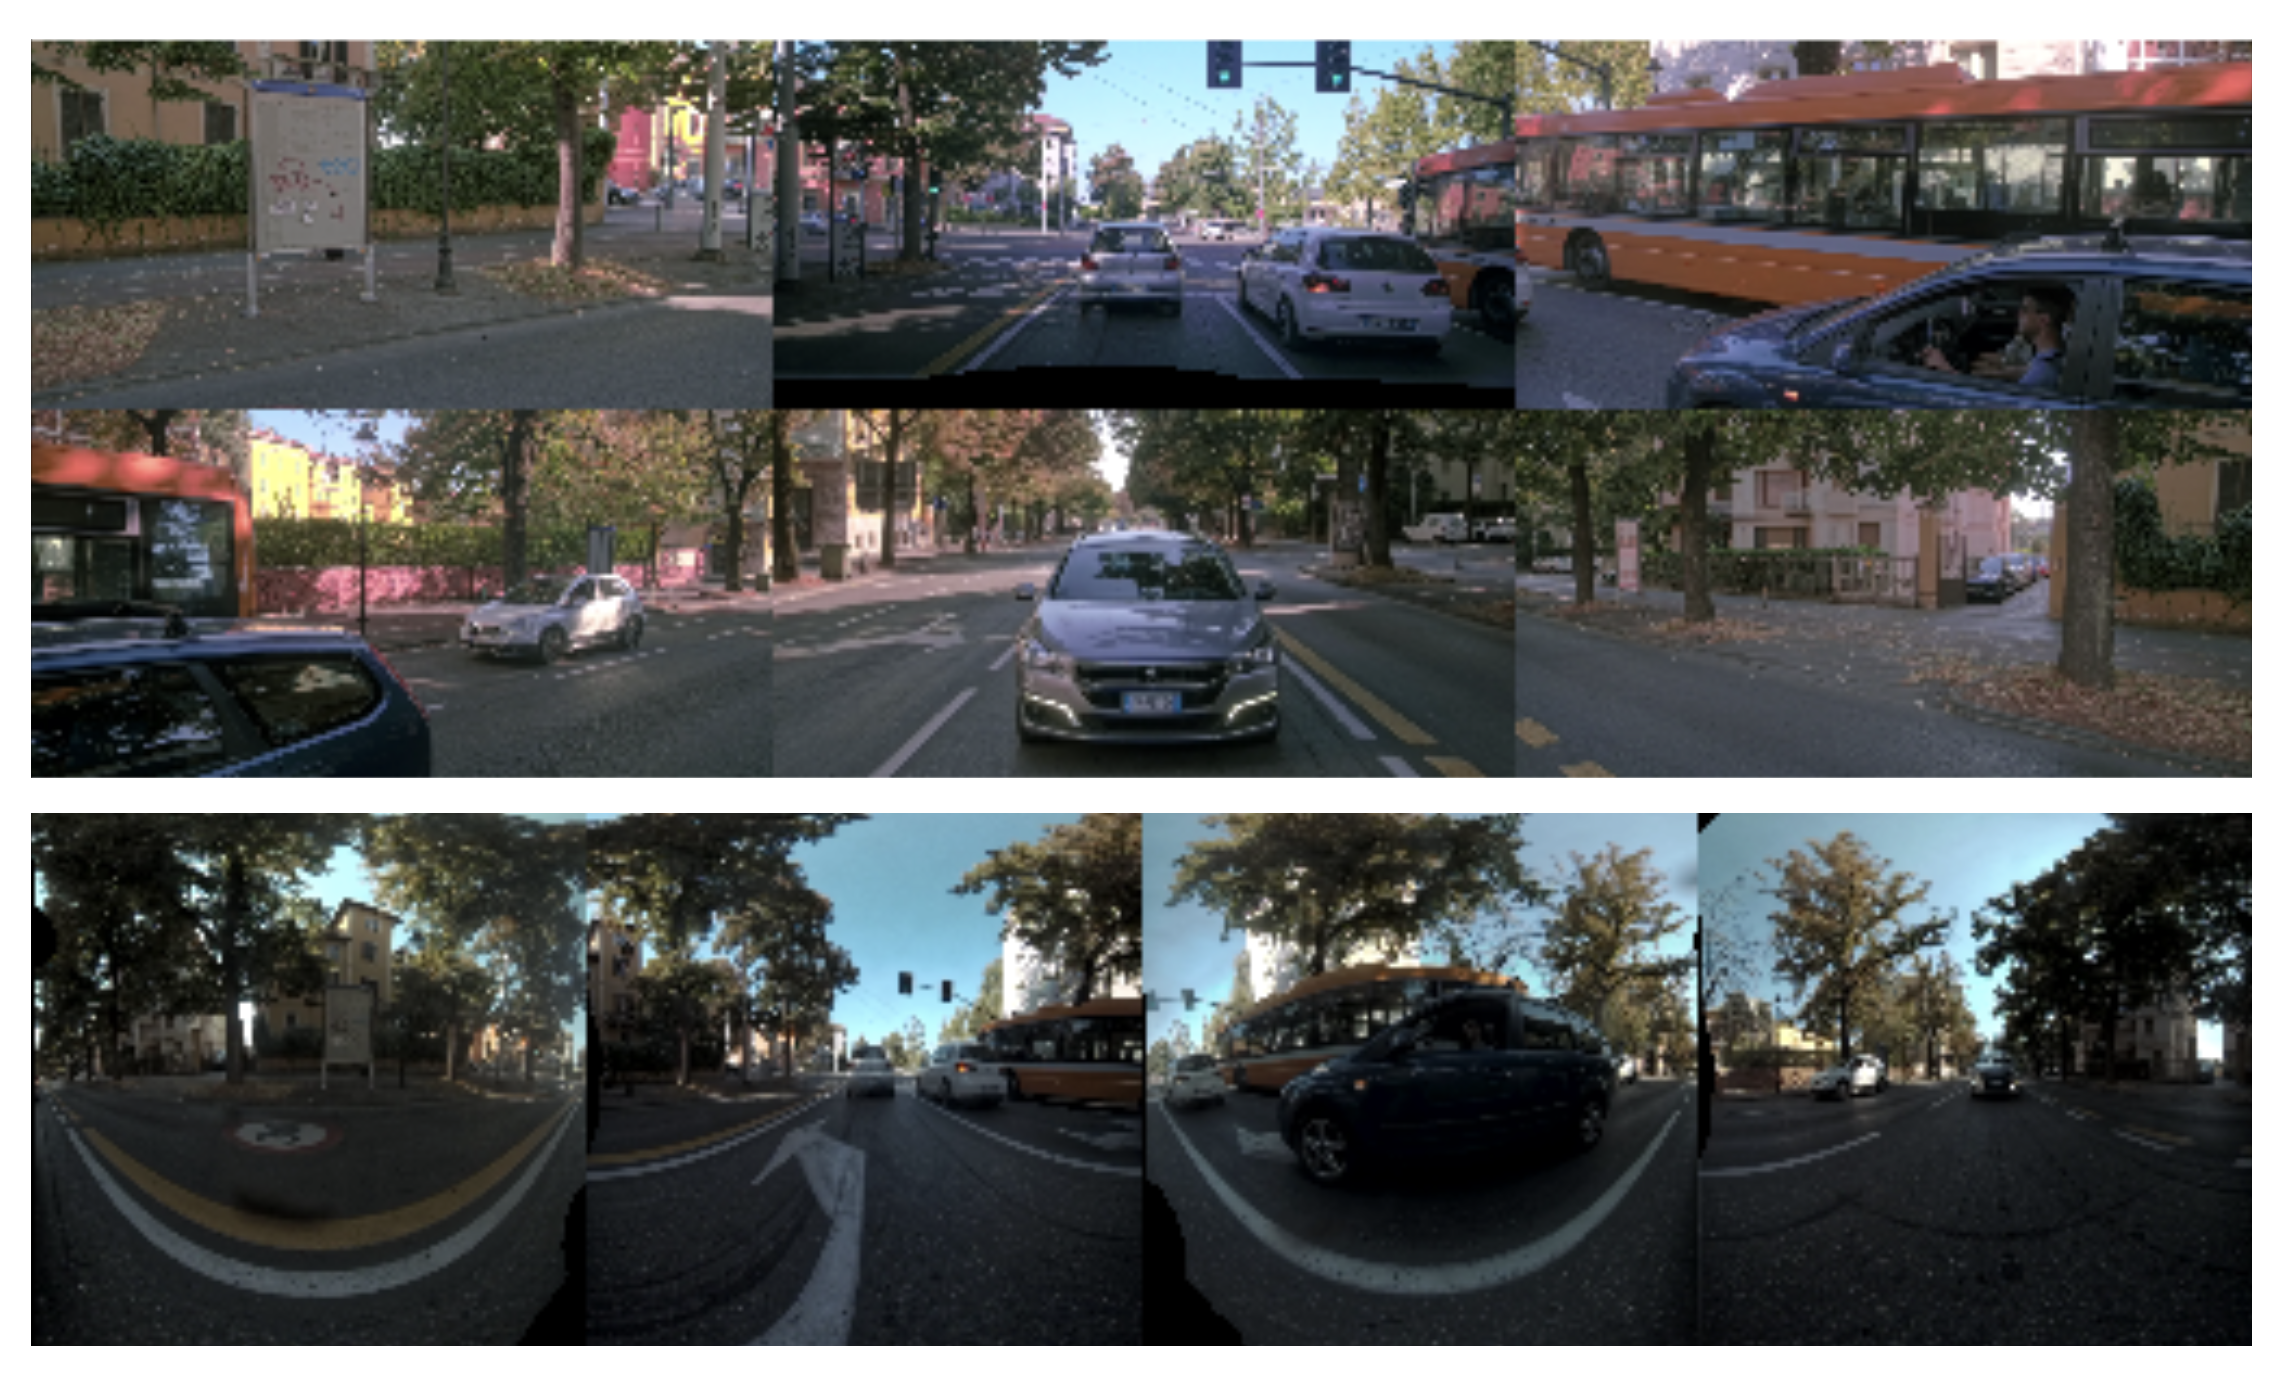
\includegraphics[width=1\linewidth]{LateX//figs/Screenshot 2024-09-27 at 12.00.55.png}
    \caption{Enter Caption}
    \label{fig:enter-label}
\end{figure}

\susubsection{HorizontalFOVLoader}
da quanto riesco a capire, ma anche per questo sarà meglio farsi spiegare, crea the horizontal FOV mask of the camera projected on the BEV.

Il codice che hai fornito definisce un loader di input per la FOV orizzontale (Horizontal FOV Loader), specificamente per un sistema che utilizza dati di telecamere per rappresentazioni bird's-eye view (BEV). Questo loader è utilizzato per caricare e calcolare campi di vista orizzontali delle telecamere (FOV, Field of View) e inserirli in un formato utile per un modello di apprendimento automatico. Qui ti spiego nel dettaglio le varie parti del codice:

1. Inizializzazione della classe HorizontalFOVLoader
Classe: La classe HorizontalFOVLoader estende BevInputLoader, che è presumibilmente un'altra classe che gestisce input per BEV.
Configurazione: Il costruttore accetta un parametro cfg che rappresenta la configurazione del sistema, solitamente estratta da un file YAML.
Vengono definite due liste di telecamere: $long_cams$ (telecamere con FOV lungo) e $short_cams$ (telecamere con FOV corto), in base alle specifiche nel file di configurazione.
Si calcolano le dimensioni delle immagini generate dalle telecamere ($long_cam_h$, $long_cam_w$, $short_cam_h$, $short_cam_w$).
Viene configurata la dimensione della vista dall’alto ($bev_h$, $bev_w$) e un parametro booleano $attend_invalid$, che indica se gestire o meno le regioni "non valide" nella proiezione.
2. Metodo $__call__$
Questo metodo viene chiamato quando si esegue un'istanza di HorizontalFOVLoader con dati di input.

Input: $frame_data$ è un dizionario che contiene i dati da elaborare, presumibilmente caricato da un file di serializzazione.
Output: Il risultato è un dizionario che contiene informazioni sul campo visivo orizzontale (FOV) per diverse telecamere:
Calcola il campo visivo orizzontale per le telecamere "long" e, se ci sono telecamere "short", anche per queste.
Se l'opzione $attend_invalid$ è attivata, gestisce i pixel non validi all'interno dei dati.
Il risultato finale è un dizionario contenente i tensori con i campi visivi (FOV) elaborati.

3. Metodo $load_hfov$
Questo metodo carica i campi visivi orizzontali (FOV) da dati specifici della telecamera e li prepara per l'elaborazione.

Seleziona i dati delle telecamere (a seconda che siano "long" o "short").
Per ogni telecamera, chiama $create_cam_hfov$ per generare una maschera del FOV (basata sui dati di calibrazione e sulla dimensione dell'immagine).
Ridimensiona il FOV per adattarsi alla dimensione della vista dall’alto e restituisce il risultato come un tensore.
4. Metodo $create_cam_hfov$
Questo metodo crea un tensor di FOV per una telecamera specifica.

Inizializza un array numpy di zeri ($hfov_tensor$) che rappresenta l'immagine BEV per il campo visivo.
Se sono disponibili sia la calibrazione della telecamera che le dimensioni dell'immagine, viene chiamato $draw_fov$ per disegnare effettivamente il campo visivo sul tensor.
L'array viene convertito in un tensore torch di tipo booleano.
5. Metodo $draw_fov$
Questo metodo effettua il calcolo geometrico per disegnare il campo visivo orizzontale (FOV) di una telecamera sulla proiezione BEV.

Calcola l'angolo di FOV della telecamera usando i parametri di calibrazione (come ku e kv, che probabilmente rappresentano fattori di scala ottica).
Calcola due direzioni che delimitano il campo visivo, rappresentate da vettori.
Disegna il campo visivo proiettando i raggi dalle direzioni calcolate e riempiendo l'area tra questi raggi in una maschera (nel caso di telecamere "long").
Per telecamere "short", il campo visivo viene disegnato come un'ellisse.
6. Struttura generale e utilizzo
Il loader calcola maschere che rappresentano le aree visibili (in termini di campo visivo) per ogni telecamera "long" e "short". Queste maschere vengono poi passate ad altre parti del sistema, probabilmente per essere utilizzate in compiti di percezione, come il rilevamento di ostacoli o l'identificazione di segnaletica stradale in un ambiente di guida.

Riassunto delle funzioni principali:
Configurazione delle telecamere: Seleziona le telecamere attive e determina la dimensione della proiezione BEV.
Caricamento dei dati delle telecamere: Per ogni telecamera, carica e calcola i campi visivi orizzontali (FOV).
Proiezione e disegno del FOV: Usa geometria per proiettare i campi visivi delle telecamere sulla mappa BEV.

\subsubsection{BEVWarpLoader}


quello che fa questa parte di codice alla fine non è altro che andare ad applicare augmentation quando è richiesta, altrimenti non viene neanche considerato. Essenzialmente quinid applica una traslazione ai dati che hanno formato la BEV. 

\subsubsection{CamPosLoader}
si tratta di un loader che in sintesi carica tutti i dati di calibrazione delle camere, tra cui gli intrinseci e gli estrinseci. 
Magari fare un piccolo accenno a che parametri sono gli estrinseci e gli intrinseci in modo da sapere esattamente il loro funzionamento all'interno della ricostruzione BEV.


\subsubsection{DirVectorLoader}
Unprojected image coordinates
(i.e. direction vector from origin of camera to the image plane at depth 1)
In other words, there are the world coordinates of pixels projected with depth=1

\subsubsection{Merge}
Merging everything together, we can obtain this image which is the real input of the network. It has to be considered that there are a lot of channels each one representing information coming from different sensors. 
\begin{figure}
    \centering
    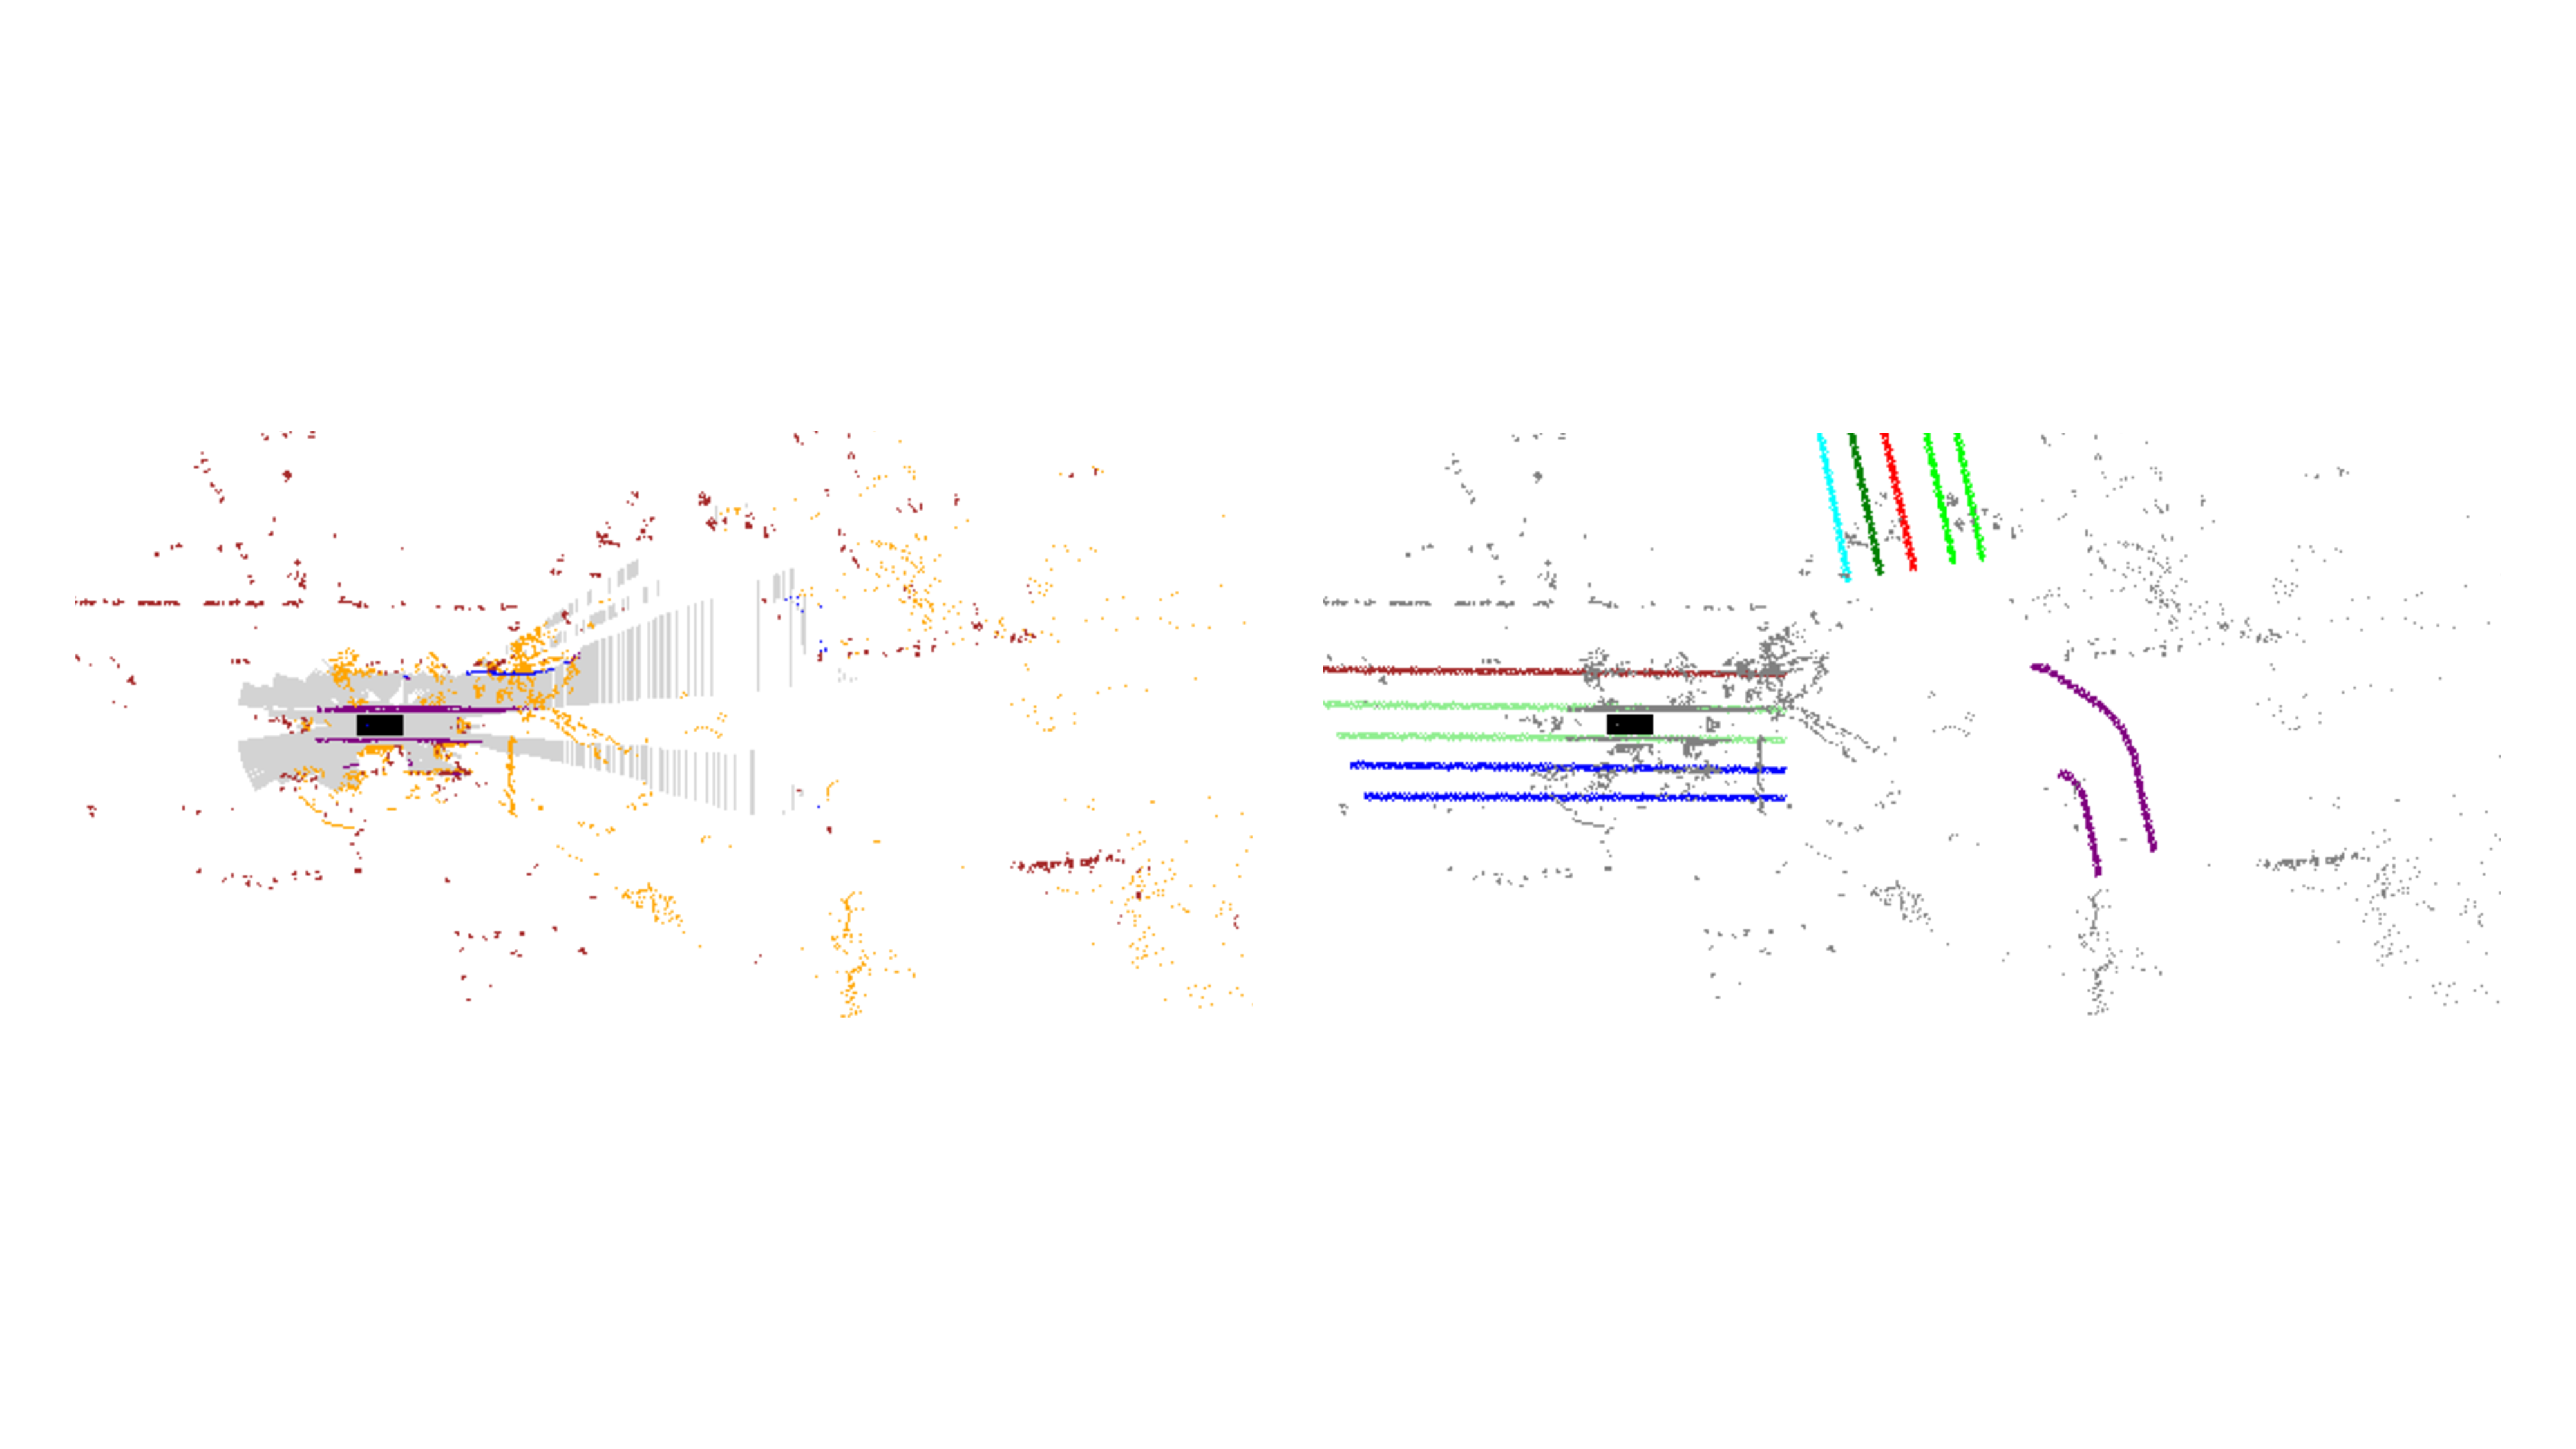
\includegraphics[width=1\linewidth]{LateX//figs/inputt.pdf}
    \caption{Enter Caption}
    \label{fig:enter-label}
\end{figure}


\section{BEV representation}
As depicted in (insert here the section in which the sensor suite is presented), the sensor suite is composed by 10 different cameras such as 6 long range and 4 short range. 

Bird’s Eye View (BEV) map prediction is essential for downstream autonomous driving tasks like trajectory
prediction. In the past, this was accomplished through the
use of a sophisticated sensor configuration that captured a
surround view from multiple cameras. However, in large-scale
production, cost efficiency is an optimization goal, so that using
fewer cameras becomes more relevant. But the consequence
of fewer input images correlates with a performance drop.
This raises the problem of developing a BEV perception
model that provides a sufficient performance on a low-cost
sensor setup. Although, primarily relevant for inference time
on production cars, this cost restriction is less problematic on
a test vehicle during training. Therefore, the objective of our
approach is to reduce the aforementioned performance drop
as much as possible using a modern multi-camera surround
view model reduced for single-camera inference. The approach
includes three features, a modern masking technique, a cyclic
Learning Rate (LR) schedule, and a feature reconstruction
loss for supervising the transition from six-camera inputs to
one-camera input during training. Our method outperforms
versions trained strictly with one camera or strictly with sixcamera surround view for single-camera inference resulting in
reduced hallucination and better quality of the BEV map.
FONTE:
https://arxiv.org/pdf/2409.02676


The Role of Behavioral Environment View (BEV) Representation in Autonomous Driving
In the rapidly evolving field of autonomous driving, the Behavioral Environment View (BEV) representation has emerged as a crucial component in facilitating safe and efficient navigation through complex environments. The BEV serves as a holistic framework that allows vehicles to interpret and respond to their surroundings by synthesizing data from various sensors. This approach is particularly significant given the challenges posed by dynamic urban landscapes, where the interaction of multiple agents—such as vehicles, pedestrians, and cyclists—creates a complex decision-making environment (Shalev-Shwartz & Shammah, 2020).

The effectiveness of BEV representation is substantially augmented by a comprehensive sensor suite, which in this context includes six long-range cameras and four short-range cameras. The long-range cameras are positioned to provide a wide field of view, typically covering distances of several hundred meters. This capability is vital for early detection of distant obstacles, such as vehicles, traffic signals, and road signs. The long-range cameras allow the vehicle to make informed decisions about trajectory planning, speed adjustments, and potential lane changes (Feng et al., 2021). For instance, detecting a red traffic light or a stop sign from a distance enables the vehicle to initiate deceleration well in advance, thus enhancing safety and passenger comfort.

On the other hand, the short-range cameras play a crucial role in capturing detailed information about nearby objects within a range of approximately 30 meters. This proximity is essential for detecting immediate threats, such as pedestrians who may suddenly enter the vehicle's path or cyclists maneuvering closely beside the vehicle. Moreover, short-range cameras are invaluable during low-speed maneuvers, such as parking and navigating tight spaces. They enable the vehicle to accurately assess distances to surrounding objects, significantly reducing the risk of collisions (Krause et al., 2017).

The integration of data from both long-range and short-range cameras into a cohesive BEV representation is achieved through advanced algorithms that leverage machine learning and computer vision techniques. These algorithms facilitate improved object detection, classification, and tracking, allowing the vehicle to dynamically adapt to changes in the environment. For example, the fusion of visual data with information from other sensors, such as LIDAR and radar, enhances the robustness of the BEV, leading to more accurate interpretations of the driving scene (Li et al., 2022). Such multi-sensor fusion enables the vehicle to create a comprehensive 3D model of its surroundings, which is crucial for understanding the spatial relationships between various elements.

Moreover, the BEV representation goes beyond simply providing a static overview of the environment; it captures the dynamic interactions of moving agents. By incorporating temporal data, the BEV can account for the predicted trajectories of pedestrians and other vehicles, allowing the autonomous system to make proactive decisions that mitigate potential risks (Paden et al., 2016). This predictive capability is essential for ensuring that the vehicle can navigate safely and efficiently, especially in complex urban settings where the behavior of other road users can be unpredictable.

The significance of BEV representation in enhancing situational awareness cannot be overstated. By synthesizing a wealth of visual data from the six long-range and four short-range cameras, autonomous vehicles can achieve a nuanced understanding of their environment. This advanced level of situational awareness contributes directly to the vehicle's decision-making processes, ultimately paving the way for safer and more reliable autonomous driving systems (Hawkins et al., 2019). As the technology continues to advance, the integration of BEV representation will play a vital role in overcoming the challenges of real-world navigation, ensuring that autonomous vehicles can operate effectively while minimizing risks to both passengers and pedestrians.




\section{Topological Map}

----

Da qualche parte si potrebbe andare a specificare che non viene utilizzato il topologico, spiegare quinid che cos'è e come funziona, quali sono i dati che potrebbe presentare. 
E spiegare anche come si riesce a non utilizzare.

----

Topological maps play a crucial role in the field of autonomous driving by providing a simplified representation of the road network and surrounding environment. These maps highlight the connectivity between different road segments, intersections, and obstacles, allowing autonomous vehicles to understand and navigate their surroundings effectively. Rather than focusing on precise geographic details or distances, topological maps emphasize the relationships between various elements, which is essential for decision-making algorithms in self-driving cars. For instance, they can help the vehicle determine possible paths and maneuvers based on the connections between roads and obstacles. In your research, topological maps may not have been necessary if the focus was on real-time sensor data or detailed spatial analysis, as these aspects require precise measurements of distances and locations to ensure safe and efficient navigation. Instead, your work might have leveraged other mapping techniques that prioritize accuracy over abstract relationships.




\section{Loss Functions}
Loss Functions: L1 Loss, Smooth L1 Loss, and Mean Squared Error (MSE)
Loss functions are essential components in machine learning models, as they quantify the difference between the predicted output and the actual target value. Among the most widely used loss functions are the L1 Loss, the Smooth L1 Loss, and the Mean Squared Error (MSE).

\subsection{L1 Loss (Mean Absolute Error)}
The L1 Loss, also known as the Mean Absolute Error (MAE), computes the sum of the absolute differences between the predicted values and the true values.
Mathematically, for a dataset with n samples, the L1 Loss is defined as:
\begin{equation}
   \text{L1}(y, \hat{y}) = \frac{1}{N} \sum_{i=1}^{N} |y_i - \hat{y_i}|
\end{equation}

This loss function is robust to outliers, as it applies a linear penalty to errors, assigning equal weight to small and large deviations. Consequently, it is particularly useful in applications where robustness to extreme values is required. 

\subsection{Smooth L1 Loss}
The Smooth L1 Loss is a hybrid between the L1 and L2 losses (the latter being the basis for the MSE). It introduces a piecewise function that is quadratic for small errors and linear for larger errors. This helps reduce sensitivity to outliers without the steep quadratic growth of the MSE. The Smooth L1 Loss is defined as follows:
\begin{equation}
    \text{Smooth-L1}(y, \hat{y}) = 
    \begin{cases} 
        0.5 \times (y_i - \hat{y_i})^2 & \text{if} \ |y_i - \hat{y_i}| < 1 \\
        |y_i - \hat{y_i}| - 0.5 & \text{otherwise}
    \end{cases}
\end{equation}


 
The smooth transition between the L1 and L2 behaviors ensures that moderate errors are not excessively penalized, contributing to a more stable training process in scenarios like deep neural network optimization. It is especially effective in problems where both small and large errors need to be handled gracefully.

\subsection{Mean Squared Error (MSE)}
The Mean Squared Error (MSE) is a widely adopted loss function that computes the average of the squared differences between predicted and actual values. It is given by:

\begin{equation}
    \text{MSE}(y, \hat{y}) = \frac{1}{N} \sum_{i=1}^{N} (y_i - \hat{y_i})^2
\end{equation}



Due to the squaring of errors, the MSE assigns a higher penalty to large errors compared to the L1 loss. This makes the MSE highly sensitive to outliers, as even small differences in large errors are amplified. MSE is particularly beneficial when large deviations from the target values need to be emphasized, such as in regression tasks where accuracy is critical.


In summary, each loss function has its specific use case:

L1 Loss is ideal when robustness to outliers is important, as it applies a linear penalty to errors.
Smooth L1 Loss provides a balanced approach by offering a smooth transition between L1 and MSE, which can stabilize training in deep learning models.
MSE is most useful when large errors should be penalized more significantly, but it can be prone to high sensitivity to outliers due to the quadratic growth of the penalty.
Choosing the appropriate loss function depends on the nature of the task and the characteristics of the error distribution in the dataset.




\begin{figure}
    \centering
    \includegraphics[width=1\linewidth]{LateX/figs/loss_functions_xkcd.pdf}
    \caption{Enter Caption}
    \label{fig:enter-label}
\end{figure}


---

short 1920x ecc scala 1
long  3840x ecc scala 2
fare anche un sottopragrafo sulla BEV






\section{Convolutional Neural Network (CNN)}

Convolutional Neural Network (CNN) Architecture
A Convolutional Neural Network (CNN), or ConvNet, is a specialized type of deep learning algorithm primarily designed for tasks requiring object recognition, such as image classification, detection, and segmentation. CNNs are widely employed in various practical applications, ranging from autonomous vehicles and medical imaging to security camera systems and facial recognition technologies.
CNN Structure and Principles
CNNs are architecturally distinct from traditional neural networks, as they take into account the spatial structure of data—usually images—by arranging neurons in a way that mimics the human visual cortex. The network's architecture is typically organized in layers, including convolutional layers, pooling layers, and fully connected layers, each playing a pivotal role in feature extraction and decision making.
CNNs are designed to handle 2D data (images) more efficiently than fully connected networks by utilizing convolutional operations instead of traditional matrix multiplications. This allows CNNs to process image data in a way that captures spatial hierarchies of patterns, from low-level edges to high-level features like objects or faces.
Key Components of CNNs
The basic building blocks of CNNs include:
    1. Convolutional Layers: These layers apply convolutional operations to the input data. In mathematical terms, a convolution operation is defined as:
      
       Here, f is the input and g is the kernel (or filter). For a 2D image, the convolution operation involves sliding a filter over the input image and computing the dot product between the filter and portions of the image, resulting in an activation map. The kernels are learnable parameters, allowing the CNN to automatically learn feature detectors for edges, textures, and higher-level patterns. Each filter responds to a particular feature within the input, like vertical edges or textures.
    2. Rectified Linear Unit (ReLU): ReLU applies a non-linear transformation element-wise after the convolution operation. Its mathematical formulation is simple:
       f(x)=max(0,x)
       This non-linearity allows the network to learn more complex patterns and ensures the network does not behave like a linear classifier.
    3. Pooling Layers: Pooling reduces the spatial dimensions of the activation maps while retaining important information. The most common form is max pooling, which selects the maximum value from each patch of the feature map. The formula for max pooling can be expressed as:
      
       Here, P is the pooling window, and x(i,j) represents the values within the window. Pooling contributes to translation invariance, which helps the network become more robust to variations in the input's position or scale.
    4. Fully Connected Layers: In the final layers of a CNN, fully connected layers are used to perform the actual classification. These layers take the high-level features detected by previous layers and map them to the final output, such as class probabilities in image classification tasks. This is where the network "decides" based on the features it has learned through the previous layers.
Learning and Feature Extraction
A key advantage of CNNs over traditional machine learning models, such as Support Vector Machines (SVMs) or Decision Trees, is that CNNs do not require manual feature extraction. CNNs automatically learn hierarchical representations of the data by using multiple convolutional and pooling layers to extract features at different levels of abstraction.
    • Translation Invariance: CNNs achieve translation invariance by applying the same convolutional filters across different parts of the image. This means that the network can recognize objects even if they appear in different locations within the image. This is a significant advantage over traditional methods, which often require the features to be manually engineered.
    • Hierarchical Feature Learning: In the early layers, CNNs detect low-level features like edges, corners, or textures, while deeper layers capture more abstract concepts like shapes or object parts. This hierarchical learning process is akin to how the human visual cortex processes visual stimuli, starting from simple to complex.
    • Efficiency: By using local connectivity, each neuron in the convolutional layers is connected only to a small region of the input (called the receptive field), not the entire input, making the computation much more efficient. Furthermore, the use of weight sharing in convolution layers—where the same filter is applied across different regions—reduces the number of parameters compared to fully connected networks.
CNN Architectures
Various CNN architectures have been developed to optimize performance for specific tasks. These architectures include:
    1. VGG-16: Known for its simplicity, VGG-16 uses small (3x3) convolutional filters but stacks a large number of convolutional layers, followed by fully connected layers.
    2. ResNet50: ResNet introduced the concept of residual learning, allowing the network to train very deep architectures by using skip connections that help prevent vanishing gradients.
    3. Inception (GoogLeNet): The Inception network introduced a more complex architecture where convolutional layers of different sizes are applied in parallel, allowing the network to capture features at multiple scales.
    4. EfficientNet: This model family scales both the width, depth, and resolution of networks to achieve higher accuracy with fewer parameters.
Mathematical Framework of CNNs
The core mathematical operations in CNNs can be summarized as follows:
    • Convolution: The operation that applies learnable filters to input data, extracting meaningful features.
    • Activation Function (ReLU): Introduces non-linearity after the convolution operation, allowing the network to learn complex mappings.
    • Pooling: Reduces the spatial dimensions of the feature maps, making the computation more efficient and the network more robust to variations in input.
    • Softmax Function: At the final layer, a softmax function is applied to generate the class probabilities:

      where zj represents the output of the final fully connected layer for class j, and n is the number of classes.
Applications Beyond Vision
While CNNs were originally designed for image-related tasks, they have been adapted for use in other domains, including:
    • Natural Language Processing (NLP): CNNs can be used for tasks like text classification by applying convolutional filters over word embeddings.
    • Time Series Analysis: CNNs can be applied to temporal data, capturing local dependencies between data points in time.
    • Speech Recognition: In conjunction with recurrent neural networks (RNNs) or transformers, CNNs can be employed for tasks like voice recognition or speech-to-text conversion.
Conclusion
CNNs represent a powerful tool in deep learning due to their ability to automatically and efficiently extract features from data, reducing the need for manual feature engineering. Their hierarchical, locally connected, and translation-invariant nature, coupled with their versatility across domains, make them indispensable in modern artificial intelligence applications. With advancements like ResNet and EfficientNet, CNNs continue to push the boundaries of what's possible in fields like computer vision, NLP, and beyond.


\subsection{Transformers}
The main challenge in multi-modal learning is that A first fundamental challenge is learning how to
represent and summarise multimodal data in a way that exploits the
complementarity and redundancy of multiple modalities.
The heterogeneity of multimodal data makes it challenging to construct
such representations. For example, language is often symbolic while audio
and visual modalities will be represented as signals.

FONTE:
T. Baltruˇsaitis, C. Ahuja, and L.-P. Morency (2018). “Multimodal machine learning: A survey and taxonomy”. In: IEEE transactions on pattern
analysis and machine intelligence 41.2, pp. 423–443

Translation: A second challenge addresses how to translate (map) data
from one modality to another. Not only is the data heterogeneous, but
the relationship between modalities is often open-ended or subjective.
For example, there exist a number of correct ways to describe an image
and and one perfect translation may not exist.

Fusion: A fourth challenge is to join information from two or more
modalities to perform a prediction.
For example, for audio-visual speech recognition, the visual description of
the lip motion is fused with the speech signal to predict spoken words.
The information coming from different modalities may have varying
predictive power and noise topology, with possibly missing data in at least
one of the modalities. IN questo caso si potrebbe cambiare l'esempio e fare riferimento alla rappresentazione BEV della mappa, ovvero che vanno unite tutte le rappresentazioni provenienti dai vari sensori ecc. 

Transformers were developed to solve the problem of sequence transduction, or
neural machine translation.
That means any task that transforms an input sequence into an output
sequence. This includes speech recognition, text-to-speech transformation,
etc...
For models to perform sequence transduction, it is necessary to have some sort
of memory

Recurrent Neural Networks have loops in them, allowing information to persist.
A Recurrent Neural Network can be thought of as multiple copies of the same
network, A, each network passing a message to a successor.
RNNs become very ineffective when the gap between the relevant information
and the point where it is needed become very large.
That is due to the fact that the information is passed at each step and the
longer the chain is, the more probable the information is lost along the chain.

With LSTMs, the information flows through a mechanism known as cell states.
In this way, LSTMs can selectively remember or forget things that are
important and not so important

The key to LSTMs is the cell state, the horizontal line running through the top
of the diagram.
The cell state is kind of like a conveyor belt. It runs straight down the entire
chain, with only some minor linear interactions. It’s very easy for information
to just flow along it unchanged.

The LSTM does have the ability to remove or add information to the cell
state, carefully regulated by structures called gates.
Gates are a way to optionally let information through. They are composed out
of a sigmoid neural net layer and a pointwise multiplication operation.
The sigmoid layer outputs numbers between
zero and one, describing how much of each
component should be let through.
An LSTM has three of these gates, to protect
and control the cell state.

The attention mechanism was introduced in 2014 to address the bottleneck
problem that arises with the use of a fixed-length encoding vector, where the
decoder would have limited access to the information provided by the input.
This is thought to become especially problematic for long and/or complex
sequences, where the dimensionality of their representation would be forced to
be the same as for shorter or simpler sequences.

When seeing a scene in our daily life, we will focus on the discriminative
regions, and process these regions quickly.
The above process can be formulated as:
Attention = f (g(x), x)
● g(x) can represent to generate attention which corresponds to the
process of attending to the discriminative regions.
● f (g(x), x) means processing input x based on the attention g(x) which
is consistent with processing critical regions and getting information.

Attention mechanisms can be categorised according to their data domain as
follows:
● What to attend to (channel)
● Where to attend to (spatial)
● When to attend to (temporal)

● Attention mechanisms that are hard involve adding a weight mask
between the input and output layers, which forces the network to focus on
the content of the image that needs attention.
This weight mask is a matrix of values that is manually fixed based on the
sampling probability of each location in the image.
Hence hard mechanisms are computationally non-differentiable, meaning
the deep NN cannot update its parameters through backpropagation
algorithms and must be trained through reinforcement learning.

In hard attention, the network only
gets input from a small portion of the
whole image. This portion is iteratively
chosen by the network through an
attention selection mechanism.

● Mechanisms can be categorised as soft if their learnable parameters are
trained through gradient descent and back-propagation algorithms.
Soft mechanisms consist of a matrix of weights that are differentially
computed through back-propagation of the entire network, or as a
separate training task of the weight model.
Attention mechanisms in RNN-models are more appropriately categorised
as ‘location-wise’ if the input is the entire input feature map, whereas one
in the category of ‘item-wise’ operates on explicit items in the input.

Feature maps in convolutional neural
networks are 2-D grids of activation
created by the application of a filter to
the layer below. In soft spatial
attention, different locations on these
grids are weighted the same across
feature maps.
In soft feature attention, different
feature maps are weighted differently

Query: These are vectors that represent positions or elements in the input
data. They are used to determine which parts of the input are relevant for a
given position.

FONTE: 
P. Ramachandran, N. Parmar, A. Vaswani, I. Bello, A. Levskaya, and J. Shlens (2019). “Stand-alone self-attention in vision models”. In:
Advances in neural information processing systems 32

Self-attention operates by transforming the input sequence into three vectors:
query, key, and value.
These vectors are obtained through linear transformations of the input. The
attention mechanism calculates a weighted sum of the values based on the
similarity between the query and key vectors.
The resulting weighted sum, along with the original input, is then passed
through a feed-forward neural network to produce the final output.
This process allows the model to focus on relevant information and capture
long-range dependencies.


QUI IL RESTO DELLE FONTI:
https://elly2023.dia.unipr.it/pluginfile.php/947/course/section/11808/lecture_14_2x1.pdf?time=1699954746673


\subsection{Architecture}

[TrainingEngine]: Preprocessor (BEVPreprocessor) has 0.0013M parameters                                                                                             │exiting
                  Backbone (BiSeNetV1) has 12.6314M parameters                                                                                                      │Client handler closed
                  Decoder (MultiUpsampleDecoder) has 0.0924M parameters                                                                                             │Client handler closed
                  Pose_seg_head (Head) has 0.0043M parameters                                                                                                       │The client is not connected anymore - 
                  Cam2bev (Cam2BEVUpNetSRM) has 26.4633M parameters                                                                                                 │exiting
                  Posnet (PoseNet4) has 12.7626M parameters                                                                                                         │The client is not connected anymore - 
                  Transform (Conv2d) has 0.0022M parameters                                                                                                         │exiting
                  Architecture (PoseNetBEV) has 51.9576M parameters

